% Options for packages loaded elsewhere
\PassOptionsToPackage{unicode}{hyperref}
\PassOptionsToPackage{hyphens}{url}
\PassOptionsToPackage{dvipsnames,svgnames,x11names}{xcolor}
%
\documentclass[
  letterpaper,
  DIV=11,
  numbers=noendperiod,
  oneside]{scrartcl}

\usepackage{amsmath,amssymb}
\usepackage{iftex}
\ifPDFTeX
  \usepackage[T1]{fontenc}
  \usepackage[utf8]{inputenc}
  \usepackage{textcomp} % provide euro and other symbols
\else % if luatex or xetex
  \usepackage{unicode-math}
  \defaultfontfeatures{Scale=MatchLowercase}
  \defaultfontfeatures[\rmfamily]{Ligatures=TeX,Scale=1}
\fi
\usepackage{lmodern}
\ifPDFTeX\else  
    % xetex/luatex font selection
\fi
% Use upquote if available, for straight quotes in verbatim environments
\IfFileExists{upquote.sty}{\usepackage{upquote}}{}
\IfFileExists{microtype.sty}{% use microtype if available
  \usepackage[]{microtype}
  \UseMicrotypeSet[protrusion]{basicmath} % disable protrusion for tt fonts
}{}
\makeatletter
\@ifundefined{KOMAClassName}{% if non-KOMA class
  \IfFileExists{parskip.sty}{%
    \usepackage{parskip}
  }{% else
    \setlength{\parindent}{0pt}
    \setlength{\parskip}{6pt plus 2pt minus 1pt}}
}{% if KOMA class
  \KOMAoptions{parskip=half}}
\makeatother
\usepackage{xcolor}
\usepackage[left=1in,marginparwidth=2.0666666666667in,textwidth=4.1333333333333in,marginparsep=0.3in]{geometry}
\setlength{\emergencystretch}{3em} % prevent overfull lines
\setcounter{secnumdepth}{5}
% Make \paragraph and \subparagraph free-standing
\makeatletter
\ifx\paragraph\undefined\else
  \let\oldparagraph\paragraph
  \renewcommand{\paragraph}{
    \@ifstar
      \xxxParagraphStar
      \xxxParagraphNoStar
  }
  \newcommand{\xxxParagraphStar}[1]{\oldparagraph*{#1}\mbox{}}
  \newcommand{\xxxParagraphNoStar}[1]{\oldparagraph{#1}\mbox{}}
\fi
\ifx\subparagraph\undefined\else
  \let\oldsubparagraph\subparagraph
  \renewcommand{\subparagraph}{
    \@ifstar
      \xxxSubParagraphStar
      \xxxSubParagraphNoStar
  }
  \newcommand{\xxxSubParagraphStar}[1]{\oldsubparagraph*{#1}\mbox{}}
  \newcommand{\xxxSubParagraphNoStar}[1]{\oldsubparagraph{#1}\mbox{}}
\fi
\makeatother


\providecommand{\tightlist}{%
  \setlength{\itemsep}{0pt}\setlength{\parskip}{0pt}}\usepackage{longtable,booktabs,array}
\usepackage{calc} % for calculating minipage widths
% Correct order of tables after \paragraph or \subparagraph
\usepackage{etoolbox}
\makeatletter
\patchcmd\longtable{\par}{\if@noskipsec\mbox{}\fi\par}{}{}
\makeatother
% Allow footnotes in longtable head/foot
\IfFileExists{footnotehyper.sty}{\usepackage{footnotehyper}}{\usepackage{footnote}}
\makesavenoteenv{longtable}
\usepackage{graphicx}
\makeatletter
\newsavebox\pandoc@box
\newcommand*\pandocbounded[1]{% scales image to fit in text height/width
  \sbox\pandoc@box{#1}%
  \Gscale@div\@tempa{\textheight}{\dimexpr\ht\pandoc@box+\dp\pandoc@box\relax}%
  \Gscale@div\@tempb{\linewidth}{\wd\pandoc@box}%
  \ifdim\@tempb\p@<\@tempa\p@\let\@tempa\@tempb\fi% select the smaller of both
  \ifdim\@tempa\p@<\p@\scalebox{\@tempa}{\usebox\pandoc@box}%
  \else\usebox{\pandoc@box}%
  \fi%
}
% Set default figure placement to htbp
\def\fps@figure{htbp}
\makeatother

\KOMAoption{captions}{tableheading}
\makeatletter
\@ifpackageloaded{caption}{}{\usepackage{caption}}
\AtBeginDocument{%
\ifdefined\contentsname
  \renewcommand*\contentsname{Table of contents}
\else
  \newcommand\contentsname{Table of contents}
\fi
\ifdefined\listfigurename
  \renewcommand*\listfigurename{List of Figures}
\else
  \newcommand\listfigurename{List of Figures}
\fi
\ifdefined\listtablename
  \renewcommand*\listtablename{List of Tables}
\else
  \newcommand\listtablename{List of Tables}
\fi
\ifdefined\figurename
  \renewcommand*\figurename{Figure}
\else
  \newcommand\figurename{Figure}
\fi
\ifdefined\tablename
  \renewcommand*\tablename{Table}
\else
  \newcommand\tablename{Table}
\fi
}
\@ifpackageloaded{float}{}{\usepackage{float}}
\floatstyle{ruled}
\@ifundefined{c@chapter}{\newfloat{codelisting}{h}{lop}}{\newfloat{codelisting}{h}{lop}[chapter]}
\floatname{codelisting}{Listing}
\newcommand*\listoflistings{\listof{codelisting}{List of Listings}}
\makeatother
\makeatletter
\makeatother
\makeatletter
\@ifpackageloaded{caption}{}{\usepackage{caption}}
\@ifpackageloaded{subcaption}{}{\usepackage{subcaption}}
\makeatother
\makeatletter
\@ifpackageloaded{sidenotes}{}{\usepackage{sidenotes}}
\@ifpackageloaded{marginnote}{}{\usepackage{marginnote}}
\makeatother

\usepackage{bookmark}

\IfFileExists{xurl.sty}{\usepackage{xurl}}{} % add URL line breaks if available
\urlstyle{same} % disable monospaced font for URLs
\hypersetup{
  pdftitle={Homomorphic Encryption for Developers},
  pdfauthor={Antonio Montano},
  pdfkeywords={cryptography, homomorphic encryption, RSA},
  colorlinks=true,
  linkcolor={blue},
  filecolor={Maroon},
  citecolor={Blue},
  urlcolor={Blue},
  pdfcreator={LaTeX via pandoc}}


\title{Homomorphic Encryption for Developers}
\usepackage{etoolbox}
\makeatletter
\providecommand{\subtitle}[1]{% add subtitle to \maketitle
  \apptocmd{\@title}{\par {\large #1 \par}}{}{}
}
\makeatother
\subtitle{Unlocking data privacy with powerful cryptographic techniques}
\author{Antonio Montano}
\date{2022-06-23}

\begin{document}
\maketitle

\renewcommand*\contentsname{Table of contents}
{
\hypersetup{linkcolor=}
\setcounter{tocdepth}{3}
\tableofcontents
}

\marginnote{\begin{footnotesize}

\pandocbounded{
\includegraphics[keepaspectratio]{homomorphic-encryption.webp}}

\end{footnotesize}}

\section{Introduction}\label{introduction}

Imagine you're building a healthcare app that needs to analyze patient
data stored in the cloud. Since the data is sensitive, you encrypt it
before sending it. However, every time you need to analyze the data, you
have to decrypt it, which means the data is exposed and creates a
security risk.

This is the main problem with traditional encryption systems like
RSA\footnote{The RSA algorithm is named after its inventors: Rivest,
  Shamir, and Adleman, who developed it in 1977. It is a widely-used
  asymmetric encryption method that relies on the computational
  difficulty of factoring large integers, currently enabling secure data
  transmission with a public key for encryption and a private key for
  decryption. Quantum computers can use Shor's algorithm to factor
  integers exponentially faster than classical algorithms, making RSA
  effectively insecure against quantum attacks. See: Rivest, R. L.,
  Shamir, A., \& Adleman, L. (1978). \textbf{A method for obtaining
  digital signatures and public-key cryptosystems}. \emph{Communications
  of the ACM}, 21(2), 120--126.
  \href{https://doi.org/10.1145/359340.359342}{DOI}, and Shor, P. W.
  (1994). \textbf{Algorithms for quantum computation: Discrete
  logarithms and factoring}. \emph{Proceedings of the 35th Annual
  Symposium on Foundations of Computer Science}, 124--134. IEEE.
  \href{https://doi.org/10.1109/SFCS.1994.365700}{DOI}} and
AES\footnote{The AES algorithm (Advanced Encryption Standard) is a
  symmetric encryption standard established by the National Institute of
  Standards and Technology (NIST) in 2001, based on the Rijndael cipher
  designed by Joan Daemen and Vincent Rijmen. It is widely used for
  secure data encryption due to its speed and robustness. See: Daemen,
  J., \& Rijmen, V. (1998). \textbf{Advanced Encryption Standard (AES)
  (FIPS PUB 197)}.
  \href{https://csrc.nist.gov/publications/fips/fips197/fips-197.pdf}{Downlaod}.
  AES relies on the computational difficulty of brute-forcing keys,
  which requires trying all possible key combinations. Quantum computers
  can use \textbf{Grover's algorithm}, which provides a quadratic
  speedup for searching through possible keys. Instead of taking \(2^n\)
  steps to brute-force an \(n\)-bit key, Grover's algorithm reduces it
  to approximately \(2^{n/2}\) steps. This means that AES-128 (128-bit
  keys) would have the equivalent security of a 64-bit key against a
  quantum computer, making it potentially vulnerable. AES-256 is
  considered quantum-resistant for the foreseeable future because
  Grover's algorithm would reduce its effective strength to \(2^{128}\),
  which is still computationally infeasible. See: UK National Cyber
  Security Centre. \textbf{On the practical cost of Grover's algorithm
  for AES key recovery}. \emph{Fifth PQC Standardization Conference}.
  \href{https://csrc.nist.gov/csrc/media/Events/2024/fifth-pqc-standardization-conference/documents/papers/on-practical-cost-of-grover.pdf}{Downlaod}}.
They protect data while it's stored or sent, but as soon as you need to
use the data, you have to decrypt it. It's like keeping money in a safe
but needing to take it out every time you want to count it. This
fundamental limitation makes it challenging to keep sensitive
information secure throughout its lifecycle, especially as more
applications rely on cloud computing, where the need for remote
processing is common.

Homomorphic encryption (HE) aims to solve this problem by allowing data
to remain encrypted even while it's being processed. It promises to make
the cloud much safer for storing and analyzing data, which could have
far-reaching impacts on healthcare, finance, and many other fields.
Imagine being able to calculate the average income of a group of people
without ever knowing how much any individual earns, that's the promise
of HE.

\subsection{The challenge with data
security}\label{the-challenge-with-data-security}

Even when data is encrypted and stored in the cloud, there are still
some risks:

\begin{enumerate}
\def\labelenumi{\arabic{enumi}.}
\item
  Metadata exposure: Even if the data is encrypted, cloud providers can
  still see some information:

  \begin{itemize}
  \tightlist
  \item
    When the data is accessed.
  \item
    How much data is being processed.
  \item
    Patterns of usage that could reveal some details.
  \end{itemize}

  Metadata may not contain the actual content of the data, but it can
  still provide insights that compromise privacy. For instance, frequent
  access to a medical record could imply a serious health condition,
  even if the actual diagnosis remains encrypted.
\item
  Trust issues: Cloud providers or intermediaries who have access to
  encryption keys could:

  \begin{itemize}
  \tightlist
  \item
    Access decrypted data when it's being processed.
  \item
    Keep metadata even after the service ends.
  \item
    Create privacy risks by storing information about data access, which
    could help them infer details even if the data itself is never fully
    decrypted
  \end{itemize}

  These issues highlight the importance of removing the need to trust
  third parties. HE can help solve this problem by ensuring that data
  remains encrypted, even when it's being analyzed.
\end{enumerate}

\subsection{Computing on encrypted
data}\label{computing-on-encrypted-data}

Let's say Alice has some data \(m\), and Bob has a function \(f\). Alice
wants to know the answer to \(f(m)\):

\begin{itemize}
\tightlist
\item
  Traditional approach: Alice has to share \(m\) with Bob.
\end{itemize}

\begin{figure}

\centering{

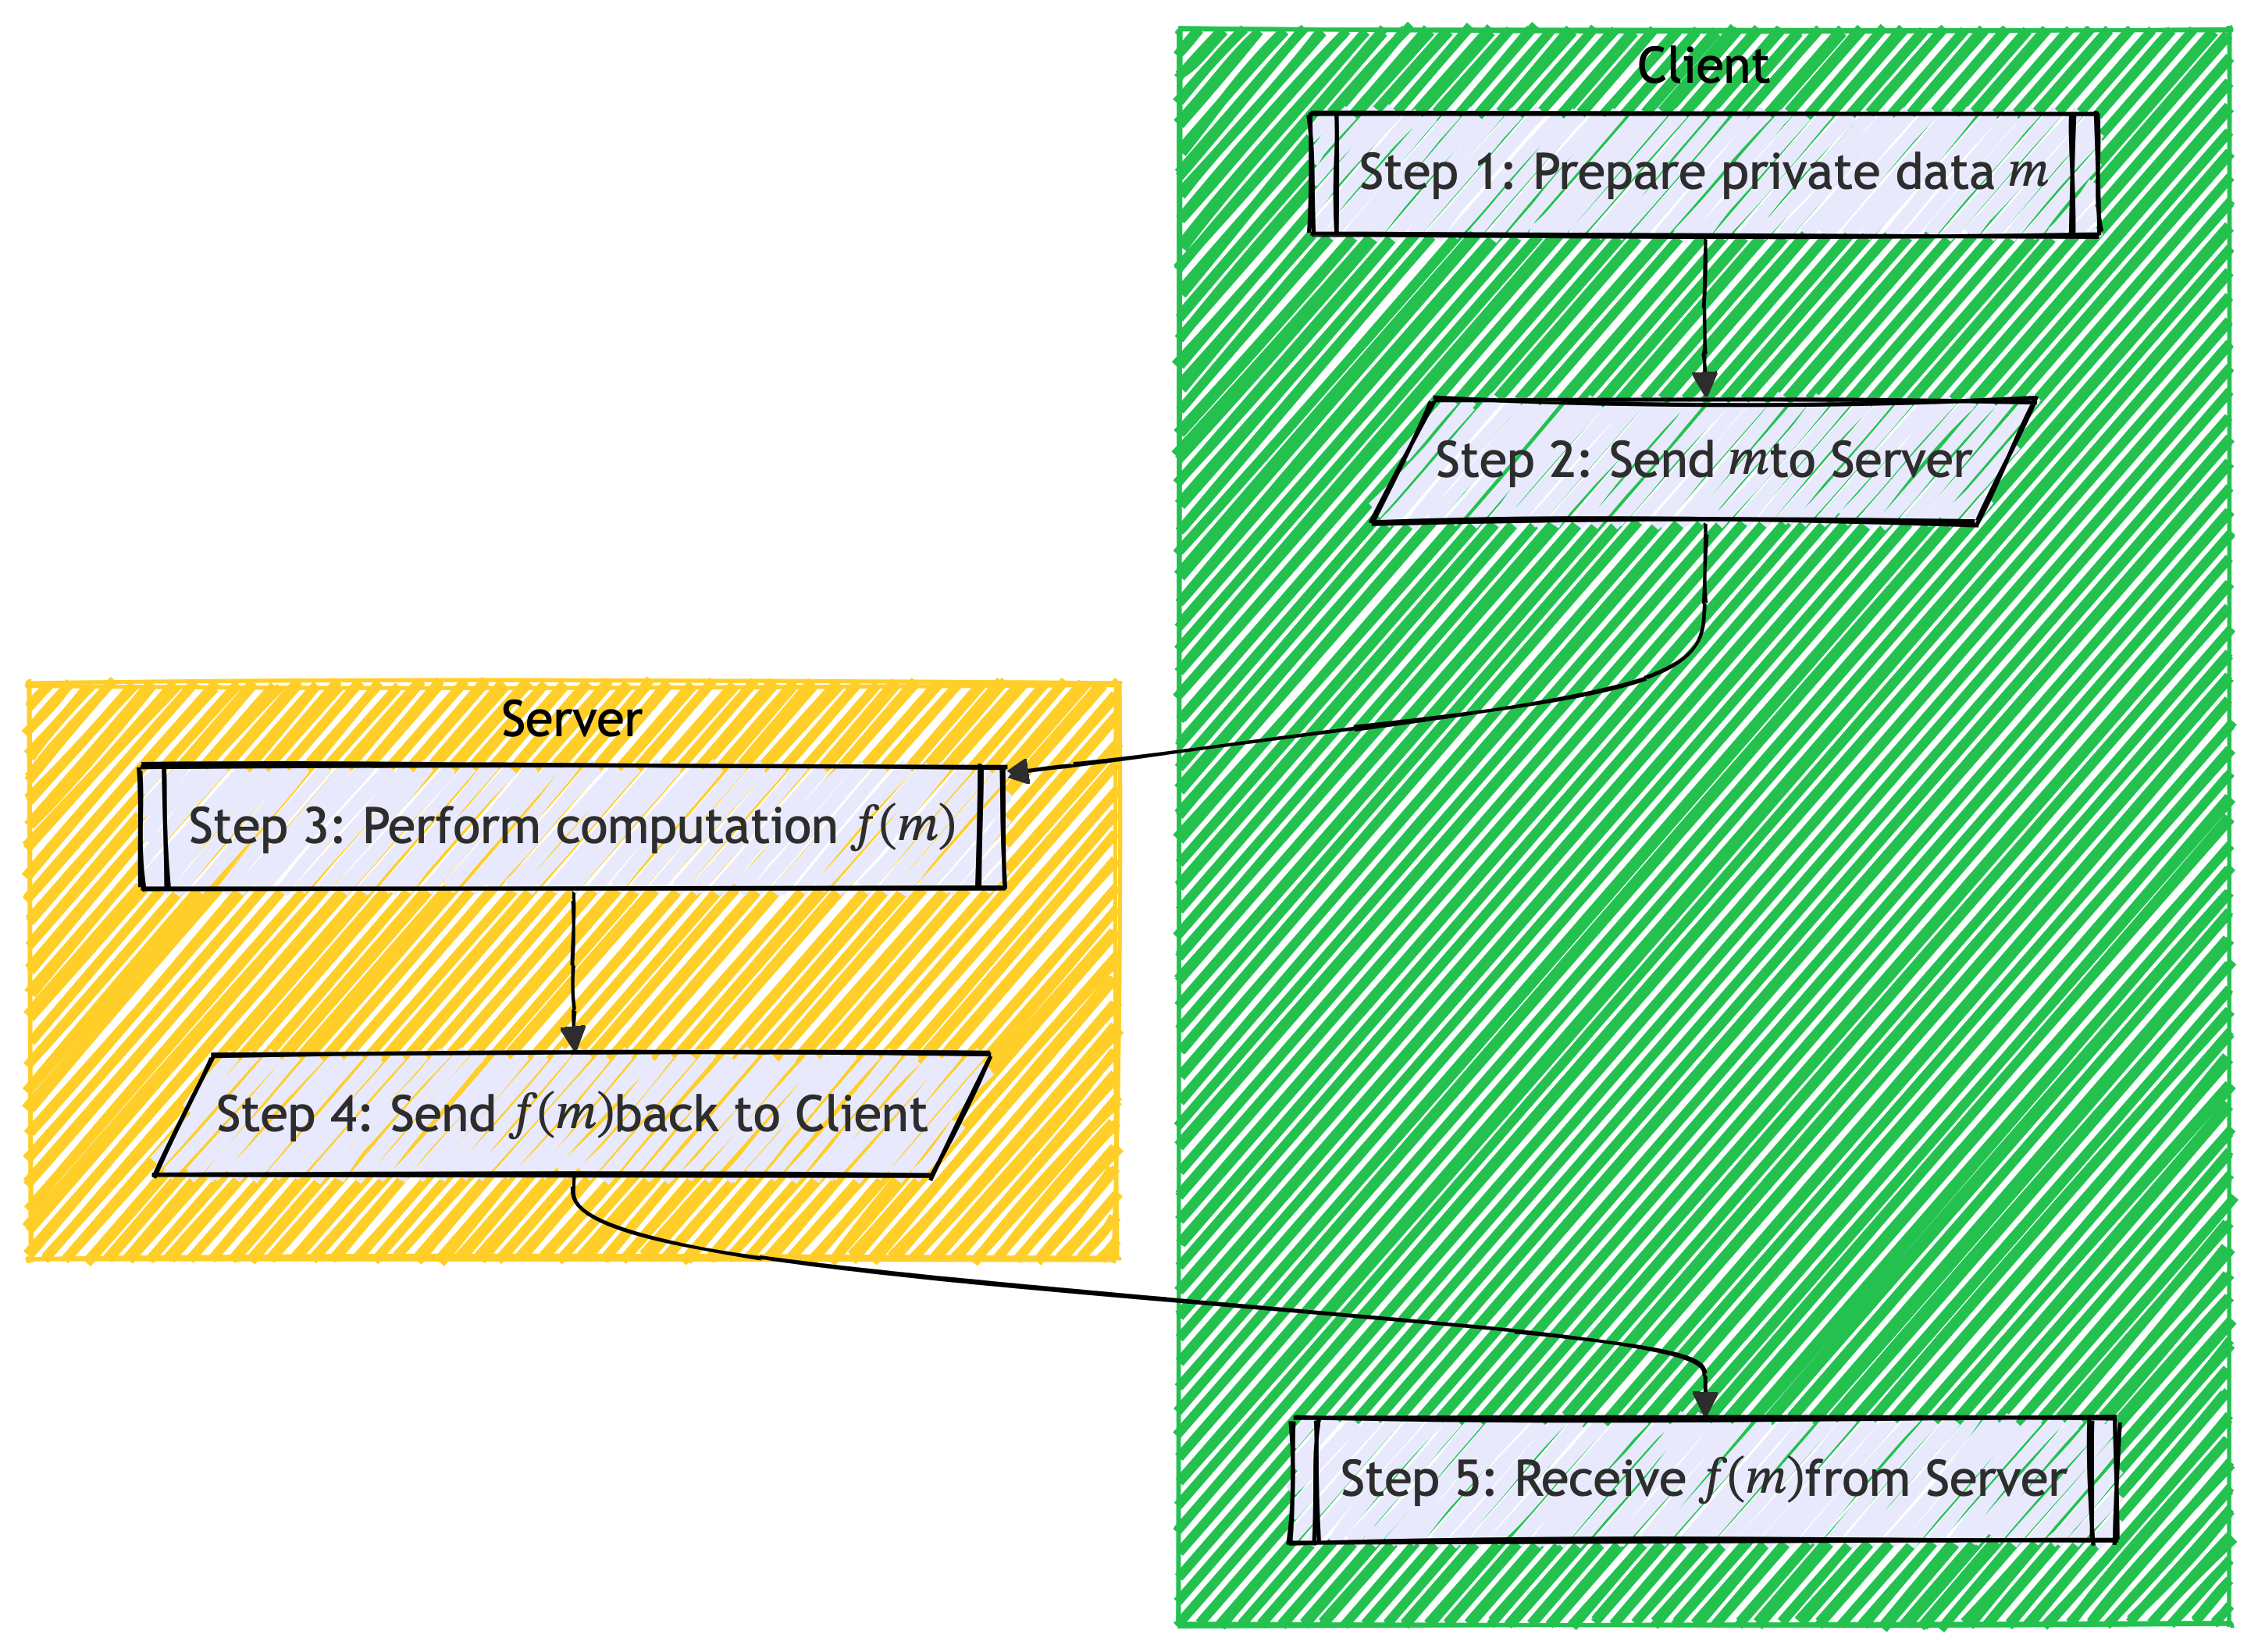
\includegraphics[width=7.52in,height=5.51in]{index_files/figure-latex/mermaid-figure-1.png}

}

\caption{\label{fig-traditional-approach-diagram}A simple client-server
scenario for the traditional approach, where C is Client (Alice) and S
is Server (Bob)}

\end{figure}%

\begin{itemize}
\tightlist
\item
  HE approach: Alice sends an encrypted version of \(m\) to Bob, and Bob
  does the calculations on the encrypted data.
\end{itemize}

\begin{figure}

\centering{

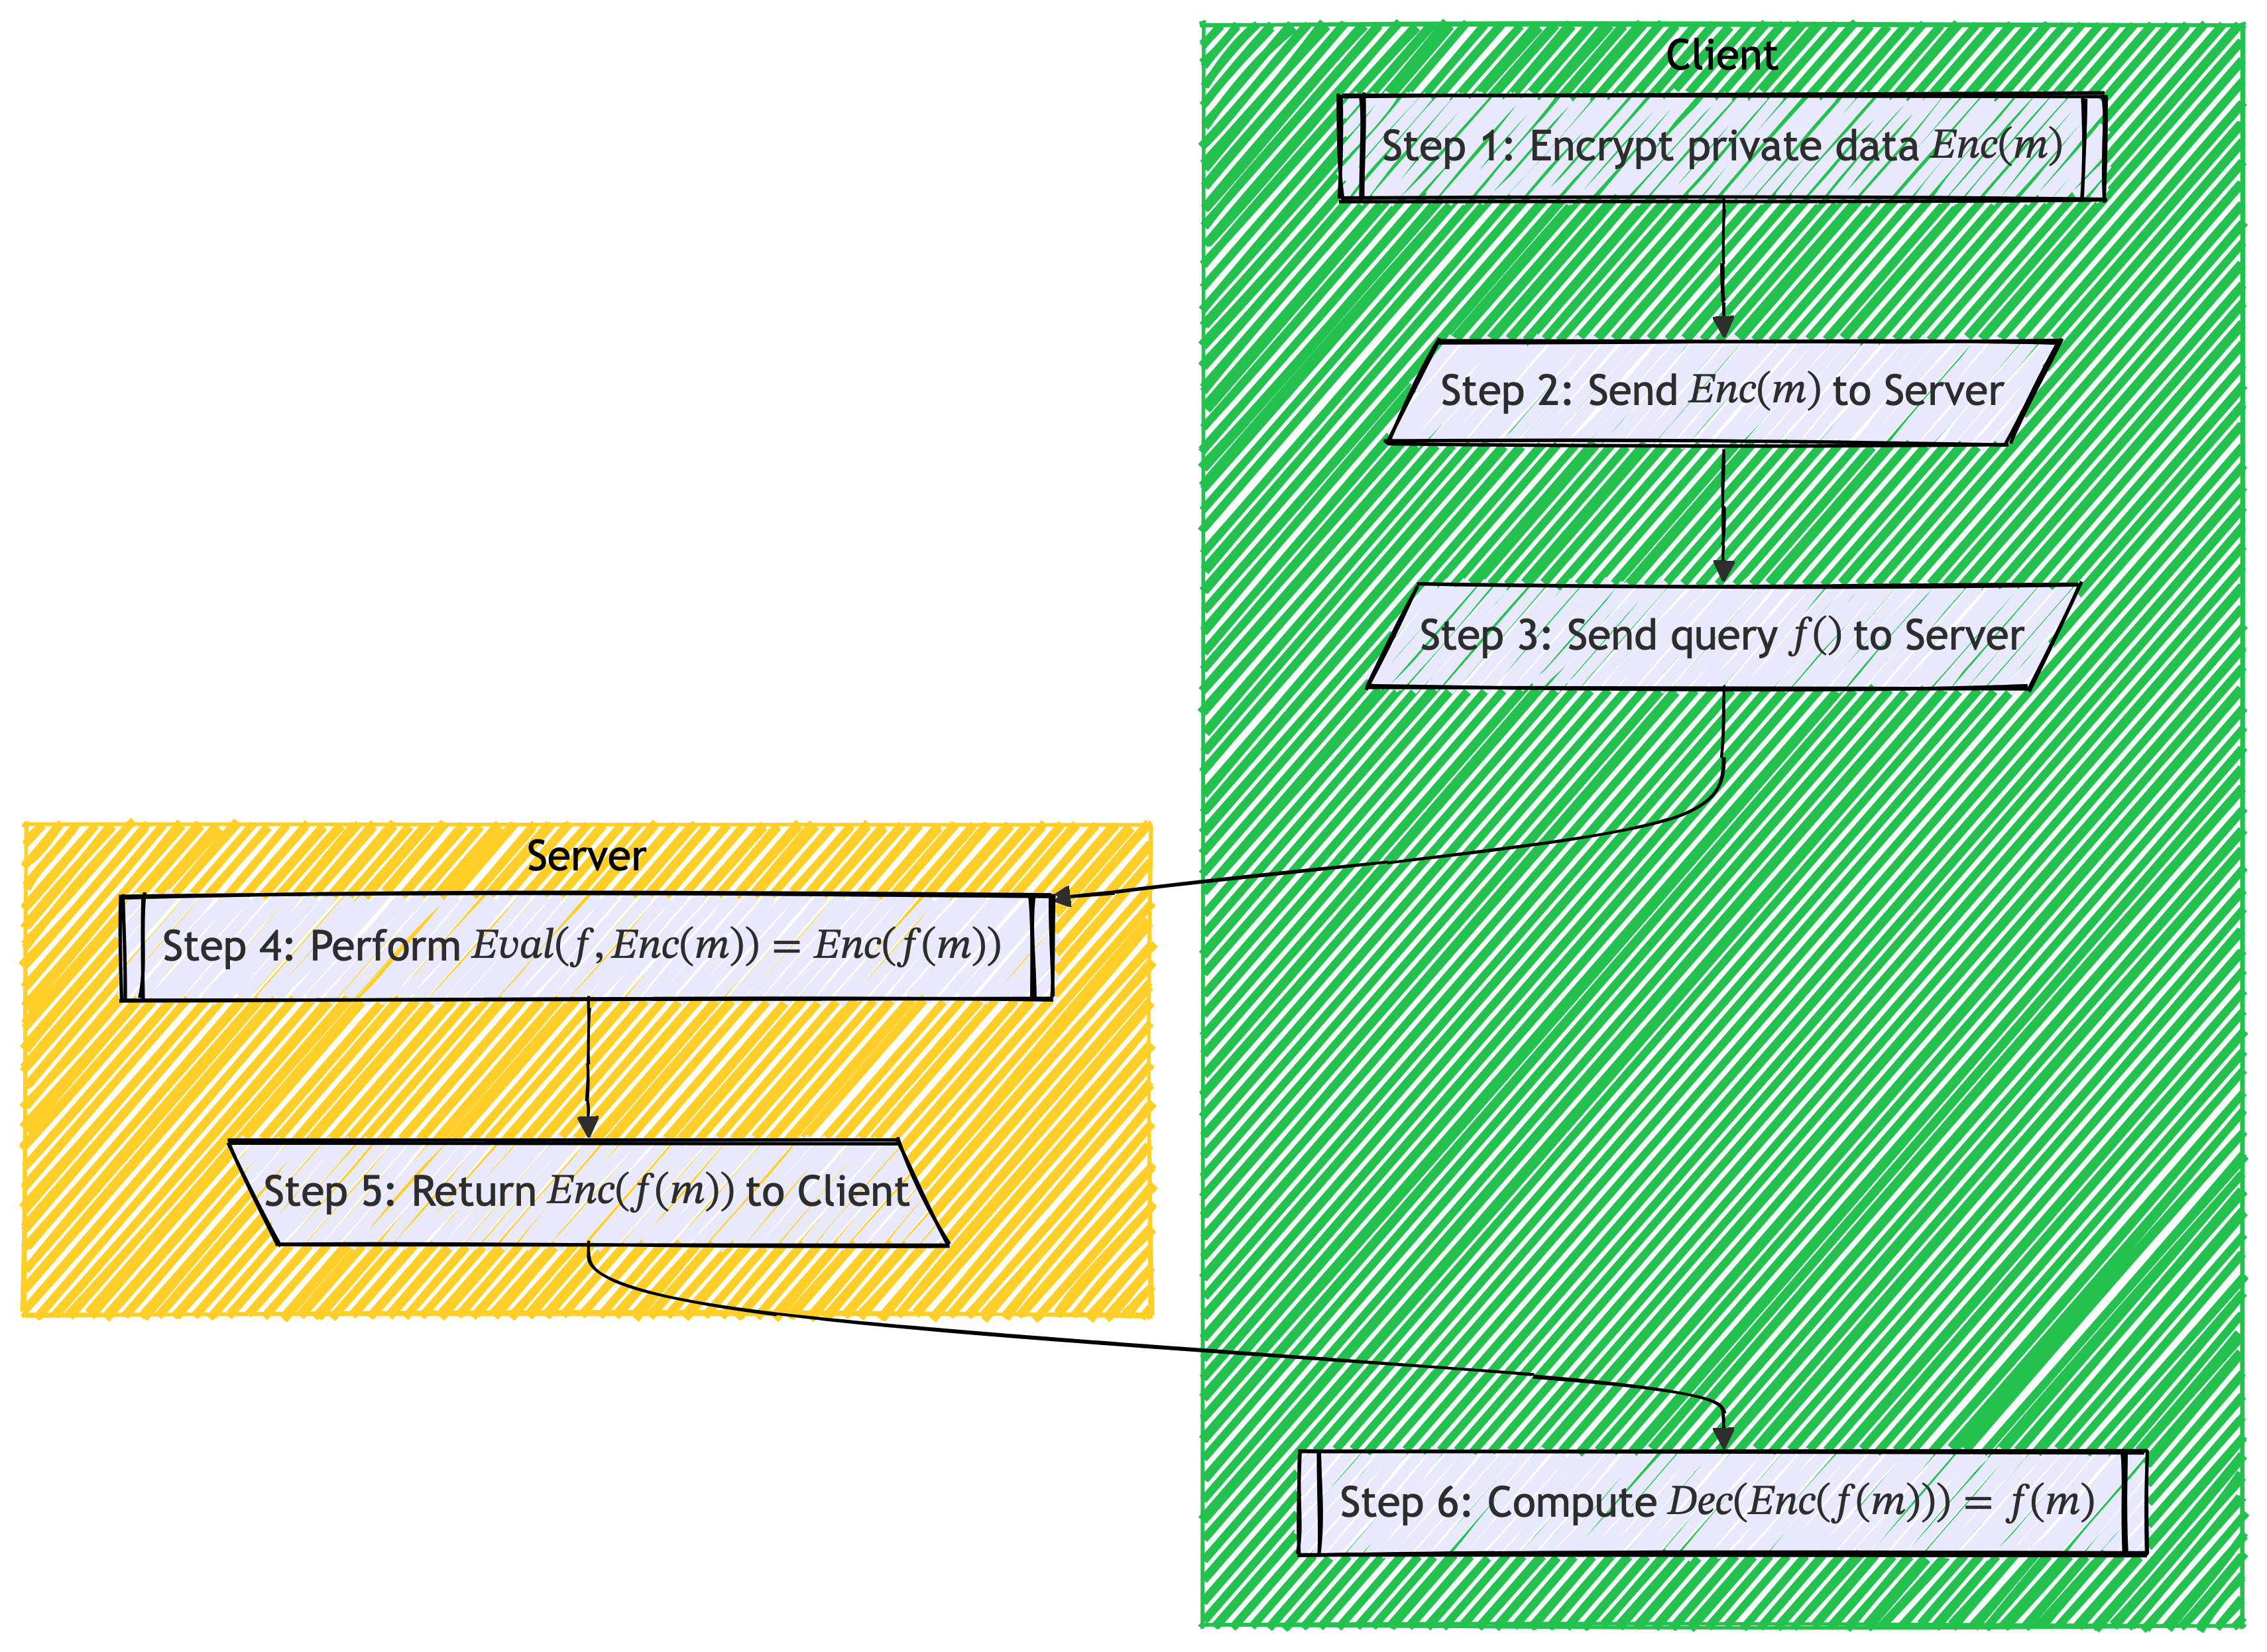
\includegraphics[width=8.8in,height=6.49in]{index_files/figure-latex/mermaid-figure-2.png}

}

\caption{\label{fig-simple-he-diagram}A simple client-server HE
scenario, where C is Client (Alice) and S is Server (Bob)}

\end{figure}%

In traditional encryption, encrypted data can't be processed in any
useful way. HE is different, because it keeps the relationships between
numbers, even when they're encrypted. Here's a simple example:

\begin{itemize}
\item
  Let's say you have two numbers, \(a\) and \(b\).
\item
  You encrypt them to get \(Enc(a)\) and \(Enc(b)\).
\item
  With HE, you can add \(Enc(a)\) and \(Enc(b)\) and get an encrypted
  result that, when decrypted, gives you \(a + b\).
\end{itemize}

This means you can perform calculations on encrypted data without having
to decrypt it first. The ability to compute on encrypted data without
decryption is what makes HE so revolutionary. In essence, it allows data
to stay secure throughout its entire lifecycle, from collection to
storage to processing.

HE works by using complex mathematical operations that preserve the
structure of the data even when it's encrypted. The mathematics behind
this is quite advanced, involving abstract algebra and number theory.
These mathematical techniques ensure that operations such as addition
and multiplication can be performed on the encrypted data in a way that
yields correct results when decrypted.

\subsection{Semantic security and controlled
malleability}\label{semantic-security-and-controlled-malleability}

HE is possible thanks to two key cryptographic concepts:
\textbf{semantic security} and \textbf{controlled malleability}. While
these might sound technical, they're not too hard to understand when
broken down.

First, let's talk about semantic security. This property ensures that
encrypted data reveals absolutely nothing about the original data. For
example, even if you encrypt the same message twice, the results will
look completely different every time, like writing a note and hiding it
in different locked boxes that look unique each time. This randomness
makes it impossible for someone to guess the original message just by
looking at the encrypted result. Semantic security is a cornerstone of
most modern encryption schemes, such as AES for secure data storage and
RSA for transmitting confidential messages over the internet. In these
systems, semantic security ensures that an attacker cannot deduce the
plaintext, even if they intercept encrypted messages.

Now, let's look at controlled malleability. Normally, encryption schemes
are designed to prevent any modification of encrypted data. For example,
in secure messaging or financial transactions, tampering with
ciphertexts could lead to corruption or malicious alterations. This is
why many encryption schemes aim to be non-malleable, ensuring
ciphertexts cannot be manipulated in any meaningful way. However, some
cryptographic protocols intentionally use a controlled form of
malleability. For instance:

\begin{itemize}
\item
  RSA encryption supports a basic level of malleability, enabling
  certain transformations (e.g., multiplying ciphertexts) that
  correspond to transformations on the plaintext. This is leveraged in
  digital signatures and secure voting systems.
\item
  Secure Multi-Party Computation (SMC) uses malleable properties to
  allow multiple parties to jointly compute a function over their inputs
  without revealing them to each other.
\end{itemize}

HE takes controlled malleability a step further by enabling a rich set
of mathematical operations, such as additions and multiplications, to be
performed directly on encrypted data. This means that encrypted data can
be actively processed, opening up new possibilities for secure
computation without exposing sensitive information.

By combining semantic security with controlled malleability, HE
represents a powerful new paradigm in cryptography. While semantic
security ensures that the original data remains completely hidden,
controlled malleability allows computations on that hidden data in a
secure and predictable way. Together, these concepts extend the
boundaries of what encryption can achieve, enabling privacy-preserving
technologies that go far beyond the limitations of traditional
cryptographic schemes.

\subsection{Types of HE}\label{types-of-he}

HE encompasses various schemes, each with distinct capabilities,
applications, and a shared mathematical heritage that connects their
evolution. These different types of HE have progressively built on one
another, with each advancement adding new capabilities while maintaining
foundational principles rooted in number theory and algebra.

\begin{enumerate}
\def\labelenumi{\arabic{enumi}.}
\item
  \textbf{Partially Homomorphic Encryption (PHE):}

  \begin{itemize}
  \item
    PHE supports a single type of operation, either addition or
    multiplication, on encrypted data, which offers high efficiency due
    to its limited operational scope.
  \item
    Applications: Ideal for scenarios requiring only one type of
    computation. For instance, PHE is utilized in secure voting systems,
    where votes are encrypted and then aggregated (added) without
    decryption, ensuring voter privacy and data integrity.
  \item
    Historical context: The concept of PHE dates back to 1978 with the
    introduction of the RSA algorithm, which supports multiplicative
    homomorphism. Subsequent schemes, such as the Paillier cryptosystem
    introduced in 1999, provided additive homomorphism, allowing for the
    addition of encrypted values. These early approaches laid the
    mathematical foundation for later, more complex forms of HE. The
    development of RSA was also a part of broader cryptographic
    breakthroughs in public-key cryptography, which fundamentally
    changed secure communication by allowing encryption without
    pre-shared keys.
  \item
    Some notable examples:

    \begin{itemize}
    \tightlist
    \item
      RSA: Supports multiplication as the homomorphic operation.
    \item
      Paillier: Addition.
    \item
      ElGamal: Multiplication.
    \item
      Goldwasser-Micali: XOR.
    \item
      Okamoto-Uchiyama: Addition.
    \end{itemize}
  \end{itemize}
\item
  \textbf{Somewhat Homomorphic Encryption (SWHE):}

  \begin{itemize}
  \item
    SWHE enables both addition and multiplication operations but only up
    to a certain depth or number of operations. It balances between
    operational flexibility and computational efficiency, making it
    suitable for applications with limited computational requirements.
  \item
    Applications: SWHE is applied in secure data aggregation, where a
    limited number of operations are performed on encrypted data to
    compute aggregate statistics without exposing individual data
    points.
  \item
    Historical context: SWHE schemes emerged as researchers sought to
    extend the capabilities of PHE. By building on the foundational
    mathematics of PHE, these schemes introduced the ability to perform
    both additive and multiplicative operations, though with certain
    limitations. This progression marked an important step towards
    achieving fully HE. The development of SWHE was influenced by
    lattice-based cryptography, which also played a crucial role in
    providing security against quantum computing attacks, linking SWHE
    to advances in post-quantum cryptography.
  \end{itemize}
\item
  \textbf{Fully Homomorphic Encryption (FHE):}

  \begin{itemize}
  \item
    FHE allows an unlimited number of both addition and multiplication
    operations on encrypted data. While computationally intensive, FHE
    provides the most comprehensive functionality, enabling complex
    computations on encrypted datasets.
  \item
    Applications: FHE is particularly valuable in privacy-preserving
    data processing, such as performing machine learning algorithms on
    encrypted medical records, allowing for data analysis without
    compromising patient confidentiality.
  \item
    Historical context: The concept of FHE was first realized by Craig
    Gentry in 2009\footnote{Gentry, C. (2009). \textbf{Fully homomorphic
      encryption using ideal lattices}. \emph{Proceedings of the 41st
      Annual ACM Symposium on Theory of Computing}, 169--178.
      \href{https://doi.org/10.1145/1536414.1536440}{DOI}}, marking a
    significant advancement in cryptography. Gentry's construction built
    upon the principles and challenges addressed by PHE and SWHE,
    demonstrating that it was possible to perform arbitrary computations
    on encrypted data without decryption. This breakthrough opened new
    avenues for secure data processing, rooted in the same mathematical
    lineage that began with PHE. Gentry's work was heavily influenced by
    the concept of ideal lattices and the use of bootstrapping, which
    allowed for refreshing encrypted data, a concept that is closely
    related to error correction techniques used in coding theory. FHE
    also contributed to advancements in multi-party computation and
    secure function evaluation, highlighting its relationship with other
    cryptographic fields focused on secure collaborative computing.
  \end{itemize}
\end{enumerate}

\subsection{How HE enhances private
computing}\label{how-he-enhances-private-computing}

HE can be combined with other privacy techniques to keep data secure
while still being able to use it. These techniques are independent but
can work well together with HE to achieve privacy goals:

\begin{itemize}
\item
  \textbf{Differential Privacy (DP)}: DP\footnote{Dwork, C., \& Roth, A.
    (2014). \textbf{The algorithmic foundations of differential
    privacy}. \emph{Foundations and Trends in Theoretical Computer
    Science}, 9(3--4), 211--407.
    \href{https://doi.org/10.1561/0400000042}{DOI}} is a method that
  ensures individual data points in a dataset can't be identified, even
  if the results are analyzed multiple times. By adding noise to the
  output, DP protects people's privacy while still allowing useful
  insights to be gained from the data. HE can be combined with DP to
  keep data encrypted during analysis, while DP adds another layer of
  privacy. For example, a healthcare company could use HE to compute
  encrypted patient data and add DP to ensure that the output does not
  compromise individual identities.
\item
  \textbf{Secure Multi-Party Computation (SMC)}: SMC\footnote{Yao, A. C.
    (1982). \textbf{Protocols for secure computations}. \emph{23rd
    annual symposium on foundations of computer science (SFCS 1982)}
    (pp.~160-164). IEEE.
    \href{https://doi.org/10.1109/SFCS.1982.38}{DOI}} allows several
  parties to jointly compute a result from their inputs without
  revealing those inputs to each other. HE is often used in SMC to make
  sure the data stays encrypted throughout the computation. This way,
  everyone can contribute without giving up their private data. For
  example, multiple banks could jointly analyze data to detect fraud
  patterns without sharing individual customer information.
\item
  \textbf{Zero-Knowledge Proofs (ZKPs)}: ZKPs\footnote{Goldwasser, S.,
    Micali, S., \& Rackoff, C. (1989). \textbf{The knowledge complexity
    of interactive proof systems}. \emph{SIAM Journal on computing},
    18(1), 186-208. \href{https://doi.org/10.1137/0218012}{DOI}} are a
  way to prove that a statement is true without revealing any other
  information beyond the fact that the statement is true. ZKPs can be
  combined with HE to verify computations on encrypted data without
  revealing any sensitive information. This is particularly useful in
  scenarios like blockchain, where privacy and verification are both
  important. For instance, ZKPs could allow someone to prove they have
  enough funds for a transaction without revealing their exact account
  balance.
\end{itemize}

\subsection{Applications of HE}\label{applications-of-he}

\subsubsection{Public cloud services}\label{public-cloud-services}

Imagine a giant digital library that many people share---this is
essentially what a public cloud service is. Services like Google Drive,
Dropbox, Microsoft Azure, or any Software as a Service (SaaS)
application, such as email platforms, social networks, or collaboration
tools, are examples where many users store and process their data in the
same place. It's like having your personal locker in a public
gym---while you have your private space, you're still using a shared
facility. The more ``layers'' or services your data interacts with, the
greater the privacy risks become, as each layer can potentially expose
your data to further vulnerabilities.

The challenge with public clouds is keeping your information private
while still being able to use all the helpful features they offer. Think
about it like this: you want to ask someone to count your money, but you
don't want them to see how much you have. That's where HE comes in: it
lets the cloud service work with your data without actually seeing
what's in it.

Public cloud services are used for various purposes, including data
storage, file sharing, and running applications remotely. The privacy
challenge in public cloud services is significant, as many users want
the benefits of powerful processing without sacrificing the
confidentiality of their data. HE offers a groundbreaking solution,
allowing computations to be performed while the data remains encrypted.
This means users can get useful insights and results from their data
without exposing it to the cloud provider or any unauthorized third
party.

HE enables users to make the most of public cloud services without
giving up their privacy. For example, organizations can store and
process customer information, health records, and financial data without
ever exposing sensitive information. This capability makes public cloud
services more secure and suitable for a wide range of applications
involving confidential data. Additionally, HE can help governments,
businesses, and individuals alike to harness the full potential of
cloud-based services without the fear of privacy breaches.

Moreover, HE provides a way for SaaS applications like email platforms
and social networks to perform useful functions on user data while
maintaining privacy. For instance, an email service could filter spam
emails or provide automated categorization features without actually
accessing the content of your emails. Similarly, a social network could
analyze user preferences to deliver targeted content or enhance user
experience, all while keeping personal data fully encrypted.

When using SaaS applications, data often passes through multiple
``layers'' of services, each adding to the potential privacy risks.
These layers could involve data storage, processing, and analysis, all
of which need to be handled with the utmost care. HE mitigates these
risks by ensuring that data is encrypted throughout its entire
journey---from storage to computation. This makes public cloud services
and SaaS platforms much safer environments for processing sensitive
information, as the data remains encrypted at every stage.

Real-world examples:

\begin{itemize}
\item
  Navigation apps: Helps you find your way without revealing where you
  are. Imagine telling someone, ``I'm somewhere in New York'' and
  getting directions without revealing your exact street corner. The
  privacy benefit is that your location stays secret while still getting
  accurate directions. HE allows navigation services to process your
  location data while keeping the exact coordinates hidden, ensuring
  your privacy while still providing efficient route guidance. This is
  especially important for users who are concerned about sharing their
  real-time location with third parties.
\item
  Health monitoring Devices: Your smartwatch or fitness tracker can
  process your health data securely. It's like having a doctor analyze
  your health charts while they're in a sealed envelope. You get health
  insights while keeping your personal metrics private. Imagine that a
  health service aggregates data from thousands of users' fitness
  trackers to find patterns in sleep quality. HE allows this analysis
  while keeping every user's specific sleep data private, so the service
  can improve recommendations without compromising privacy. This means
  that even if the cloud service processes millions of health records,
  individual users' data remains secure and confidential.
\item
  Personal finance: Gets insights from your data without exposing the
  details. Similar to having someone tell you if your spending is normal
  for your age group without seeing your actual purchases. You learn
  from your data while keeping it confidential. A budgeting app could
  use HE to compare a user's spending habits against aggregate data to
  provide personalized recommendations, all while keeping individual
  transactions encrypted and secure. For instance, the app could analyze
  spending trends, identify areas for improvement, and suggest budgeting
  strategies---all without ever accessing your raw financial data in a
  readable form.
\item
  Email filtering: Modern email services often use filters to identify
  spam, categorize messages, and even detect potential phishing attacks.
  With HE, these services can perform all of these operations without
  having to read the content of your emails. This ensures that your
  private messages remain confidential while still benefiting from
  advanced filtering and organizational features. Imagine an email
  provider categorizing your emails into folders such as Promotions,
  Social, and Primary---all without actually knowing what the emails
  say.
\item
  Social networks: Social media platforms often use algorithms to
  suggest content based on user behavior. With HE, these platforms can
  analyze user interactions, such as likes, comments, and shares, to
  provide tailored content recommendations, all while keeping user
  behavior encrypted. For example, if a social network wants to
  recommend friends or content, it can do so based on encrypted data,
  ensuring that your activity and preferences are kept private.
\item
  Collaboration tools: SaaS collaboration tools like document editors or
  project management software can use HE to provide enhanced features
  while keeping user data private. Imagine multiple users collaborating
  on a shared document, HE can ensure that the document remains
  encrypted while allowing authorized users to make edits and comments.
  This is crucial for businesses that need to ensure confidentiality
  while leveraging the benefits of cloud-based collaboration.
\end{itemize}

HE represents a transformative approach to data privacy, particularly in
the context of public cloud services and SaaS applications. However, as
the usage of digital services continues to expand, the potential for
data misuse also grows, posing significant risks to both individuals and
companies. Data can be weaponized for malicious purposes, from targeted
disinformation to financial exploitation, and traditional privacy
measures, such as DP, may not be sufficient to fully protect sensitive
information in these evolving digital landscapes. DP, while effective at
masking individual contributions in datasets, often relies on the
careful calibration of privacy budgets and noise, which can degrade
utility or be insufficient against sophisticated attacks like
reconstruction or linkage attacks, where adversaries can leverage
external datasets to infer private information. HE, on the other hand,
offers a promising solution by enabling computation on encrypted data
without ever exposing it, providing a stronger safeguard against these
emerging threats.

\subsubsection{Private cloud computing}\label{private-cloud-computing}

Private cloud computing provides organizations with greater control over
their data and infrastructure compared to public cloud environments.
This model is particularly suitable for handling sensitive information
but requires a sophisticated, defense-in-depth approach to maintain data
privacy and security throughout its lifecycle.

Private clouds are often employed by organizations that need to comply
with stringent regulatory requirements, such as those related to
healthcare, finance, or government operations. These regulations,
including standards like HIPAA, GDPR, NIS2, and PCI DSS, mandate strict
data protection protocols and require demonstrable security controls and
audit trails.

Despite the advantages of private clouds, they remain susceptible to
various threats across different layers of the technology stack.
Infrastructure layer threats include software vulnerabilities in
virtualization platforms, hypervisors, or orchestration tools, which can
lead to risks such as privilege escalation or remote code execution
(RCE). Hardware vulnerabilities, such as side-channel attacks exploiting
cache timing, power analysis, or electromagnetic emanations, also pose
significant risks. Physical security concerns, such as cold boot attacks
and DMA attacks, along with supply chain vulnerabilities in hardware
components or firmware, further complicate the security landscape.

Network layer threats include attacks such as ARP poisoning, VLAN
hopping, and compromises of software-defined networking (SDN)
controllers. Weaknesses in virtual network functions (VNFs) and
east-west traffic attacks between workloads within the cloud are also
notable vulnerabilities.

Application layer threats involve issues like API security
vulnerabilities, container escape risks that allow attackers to move
from containers to host systems, weaknesses in securing microservice
interactions, and data leakage through application logic flaws.

Human and operational threats are also significant. Configuration drift
and misconfigurations can lead to gradual deviation from secure states,
while inadequate privilege management and insider threats (both
malicious and unintentional) can compromise security. Operational
security failures, such as lapses in maintaining secure practices, are
also critical factors that must be addressed.

To mitigate these risks, organizations need a comprehensive,
multi-layered security strategy that implements defense-in-depth through
multiple complementary technologies. HE serves as one critical component
within this broader security architecture, particularly for protecting
data confidentiality during processing. Various cryptographic and
security measures work together as follows:

\begin{itemize}
\item
  In the foundational security layer, hardware security modules (HSMs)
  are used for key management, providing secure storage and handling of
  cryptographic keys which are crucial for HE operations. Trusted
  platform modules (TPMs) ensure boot integrity, establishing a trusted
  baseline for secure operations, which is essential for protecting the
  integrity of encrypted data processed using HE. Secure boot and
  measured boot processes protect the system from boot-level attacks,
  creating a secure foundation for any HE-related operations. Physical
  security controls and monitoring provide physical safeguards for cloud
  hardware, preventing physical attacks that could compromise the
  hardware used to perform HE computations.
\item
  In the network security layer, microsegmentation with zero-trust
  principles limits lateral movement within the network, ensuring that
  even if an attacker gains access, they cannot reach the nodes
  performing HE computations. Virtual network encryption ensures data
  confidentiality across virtual networks, which complements HE by
  protecting data during transit, even before or after HE-based
  processing. Network access control with 802.1x enforces authentication
  for devices on the network, preventing unauthorized devices from
  accessing data that may be encrypted using HE. SDN security, involving
  the separation of control and data planes, helps mitigate
  vulnerabilities within SDN environments, providing a secure pathway
  for the data to be processed using HE without risking exposure.
\item
  For data in transit, Transport Layer Security (TLS) 1.3 with perfect
  forward secrecy protects data from interception, while IPsec provides
  network-level encryption, ensuring that data remains secure during
  transmission before and after HE operations. For data at rest, AES-256
  encryption with secure key management protects stored data from
  unauthorized access, complementing HE by providing strong encryption
  when data is not actively being processed. Format-preserving
  encryption is used for structured data, allowing for HE-based
  operations to occur without altering the structure of sensitive
  datasets, which is particularly useful for preserving data integrity
  while performing encrypted computations.
\item
  For data in use, HE is combined with Trusted Execution Environments
  (TEEs)\footnote{McKeen, F., Alexandrovich, I., Berenzon, A., Rozas,
    C., Shafi, H., Shanbhogue, V., \& Savagaonkar, U. R. (2013).
    \textbf{Innovative instructions and software model for isolated
    execution}. \emph{Proceedings of the 2nd International Workshop on
    Hardware and Architectural Support for Security and Privacy (HASP)}.
    https://doi.org/10.1145/2487726.2488368} for enhanced data
  protection during processing. TEEs provide a secure, isolated hardware
  environment for executing sensitive operations, protecting against
  unauthorized access by ensuring that data and computations are
  shielded from other processes on the system. HE further enhances this
  by keeping the data encrypted even within the TEE, ensuring that even
  if the secure environment is compromised, the data remains
  confidential.
\item
  SMC is also employed for collaborative computations without revealing
  individual inputs. Advanced integrations include using HE with Intel
  SGX for secure computation spaces, hybrid HE-MPC protocols for
  efficient distributed computing, and memory encryption with AMD SEV or
  Intel TDX for enhanced data protection.
\item
  HE can also be integrated with Attribute-Based Encryption
  (ABE)\footnote{Goyal, V., Pandey, O., Sahai, A., \& Waters, B. (2006).
    \textbf{Attribute-based encryption for fine-grained access control
    of encrypted data}. \emph{Proceedings of the 13th ACM Conference on
    Computer and Communications Security (CCS)}, 89-98.
    \href{https://doi.org/10.1145/1180405.1180418}{DOI}} to allow
  fine-grained access control, ensuring that data access is granted only
  to users with specific attributes or roles. Identity-Based Encryption
  (IBE)\footnote{Boneh, D., \& Franklin, M. (2001).
    \textbf{Identity-based encryption from the Weil pairing}. \emph{SIAM
    Journal on Computing}, 32(3), 586-615.
    \href{https://doi.org/10.1137/S0097539701398521}{DOI}} simplifies
  key management by allowing public keys to be derived from unique user
  identifiers, reducing the complexity of certificate distribution
  (Boneh, D., \& Franklin, M., 2001). ZKPs provide anonymous
  authentication, allowing users to prove their identity or access
  rights without revealing any underlying sensitive information. By
  combining these techniques, HE ensures that data remains encrypted
  throughout its lifecycle while still allowing flexible and secure
  access management, simplified key handling, and privacy-preserving
  authentication.
\end{itemize}

This layered approach ensures that HE is not deployed in isolation but
rather as part of a comprehensive security architecture where each
component strengthens the overall security posture. The combination of
these technologies provides defense-in-depth while addressing specific
threats at each layer of the infrastructure.

Real-world examples:

\begin{itemize}
\item
  Medical research: HE, when combined with AES-256 encryption and TEEs,
  allows hospitals to study patient data while maintaining privacy.
  Within the private cloud, patient data is securely stored using
  AES-256 encryption and processed within TEEs, while HE allows
  computations on encrypted data without decryption. For example,
  doctors can analyze medical images with patient details encrypted and
  isolated, enabling researchers to identify important patterns without
  seeing individual patient information. When data needs to be shared
  across institutions, SMC is used to ensure data privacy, thereby
  identifying effective treatments and new drug opportunities while
  ensuring patient privacy.
\item
  Financial services: In the private cloud, financial institutions store
  customer data encrypted using AES-256 and conduct computations using
  HE combined with TEEs. TLS ensures data confidentiality when it moves
  in and out of the private cloud. HE, in combination with TLS for data
  in transit and TEEs for processing, helps financial institutions
  process banking information while keeping account details secret.
  Banks can use HE to assess loan applications by running risk analyses
  on encrypted financial data within TEEs, enabling automated
  decision-making without exposing customers' financial histories. This
  combination ensures data remains confidential throughout its
  lifecycle, from transmission to analysis.
\item
  Defense sector: Within a private cloud environment, sensitive
  defense-related data is encrypted with AES-256 and processed securely
  using HE and TEEs. For example, a remote-controlled drone can perform
  target calculations using HE while ensuring that even if intercepted,
  the encrypted data and computations remain confidential, safeguarding
  operational integrity. Logistics data can also be analyzed
  collaboratively among trusted partners using SMPC without revealing
  the underlying sensitive information, ensuring data privacy and
  safeguarding national security interests. TLS and IPsec are used to
  protect data that enters or exits the private cloud, ensuring that no
  sensitive information is exposed during transmission.
\end{itemize}

\subsubsection{Blockchain technology}\label{blockchain-technology}

Blockchain technology can be thought of as a digital ledger that
everyone can see---like a giant spreadsheet that tracks transactions.
The challenge is: how do you keep certain details private on this public
ledger? It's similar to wanting to tell people you bought something
without revealing how much you paid for it.

Blockchain technology is known for its transparency and security, which
are useful for verifying transactions. However, this transparency also
creates a privacy challenge. To address this, HE, ZKPs, and SMC are
employed to protect sensitive information while maintaining the
integrity and verifiability of blockchain data.

\paragraph{HE, ZKPs, and SMC}\label{he-zkps-and-smc}

HE ensures that sensitive information remains protected throughout the
process. In blockchain systems, this is crucial for maintaining privacy
without compromising the ability to verify data integrity. For example,
HE can be used to perform operations on encrypted transaction details,
such as calculating total transaction amounts or processing smart
contract conditions, enabling stakeholders to verify outcomes without
seeing the underlying sensitive data. In privacy-focused Layer 2
solutions on Ethereum, HE can be applied to compute transaction fees or
aggregate user balances in encrypted form, maintaining both privacy and
scalability. Similarly, in blockchain-based supply chain systems, HE
enables participants to encrypt transaction details before adding them
to the blockchain, ensuring that sensitive information (like pricing or
quantities) remains hidden while the overall process can still be
verified by stakeholders. This privacy-preserving transparency is
crucial in competitive environments, allowing stakeholders to verify
product provenance without exposing confidential business information.

ZKPs are leveraged in blockchain to enhance privacy by allowing parties
to prove that certain statements are true without revealing specific
information. In supply chain scenarios, ZKPs can prove that specific
procedures were followed or quality standards were met without
disclosing proprietary details. This ensures compliance while
maintaining confidentiality. In digital identity verification, ZKPs
allow individuals to prove attributes of their identity (such as being
of legal age) without exposing their full identity or birthdate,
ensuring privacy and compliance.

SMC is leveraged to enable collaborative decision-making or data
aggregation on the blockchain without exposing individual inputs. This
is particularly useful in decentralized finance (DeFi) platforms or
voting mechanisms within decentralized governance systems. For instance,
in Decentralized Autonomous Organizations (DAOs), SMC allows members to
collectively compute outcomes (such as voting results) while keeping
individual votes private, ensuring both transparency and privacy in the
decision-making process.

Both HE and ZKPs aim to preserve privacy while proving computation
correctness. They are often used together to enhance privacy in
blockchain systems. For instance, HE can encrypt inputs while ZKPs prove
the correctness of computations on these encrypted inputs. zk-SNARKs
(Zero-Knowledge Succinct Non-Interactive Arguments of Knowledge) can
also be used to prove the correct execution of homomorphic operations,
providing efficient and verifiable computations. Hybrid protocols that
combine HE and ZKPs create efficient, private smart contracts where the
correctness of encrypted computations is guaranteed without revealing
sensitive information.

SMC and HE are complementary technologies for performing private
computations on blockchain. HE can be integrated within SMC protocols to
reduce the number of communication rounds required, leading to more
efficient computations. Hybrid protocols that combine FHE and SMC
provide improved performance and security in blockchain applications.
For example, SMC and HE are used together in threshold cryptography
implementations to enable secure collaborative decision-making and
private data aggregation, while ensuring sensitive information remains
confidential.

\paragraph{Other cryptographic
techniques}\label{other-cryptographic-techniques}

The following cryptographic techniques share a common foundation in
supporting privacy-preserving, hidden but verifiable computations on
blockchain. These methods are often combined to enhance privacy,
security, and efficiency in blockchain systems:

\begin{itemize}
\item
  \textbf{Commitment schemes and HE}: A commitment scheme\footnote{Brassard,
    G., Chaum, D., \& Crépeau, C. (1988). \textbf{Minimum disclosure
    proofs of knowledge}. \emph{Journal of Computer and System
    Sciences}, 37(2), 156-189.
    \href{https://doi.org/10.1016/0022-0000(88)90005-0}{DOI}} is a
  cryptographic protocol that allows one party to commit to a chosen
  value while keeping it hidden from others, with the ability to reveal
  the value later. It ensures both secrecy and the ability to verify the
  commitment, which is essential for many blockchain applications.
  Commitment schemes and HE support hidden but verifiable computations
  on blockchain. Homomorphic commitments allow computations to be
  performed on committed values without revealing them, which can be
  combined with HE for verifiable encrypted computations. This
  combination is particularly useful in confidential transaction
  protocols, where participants need to commit to transaction values
  while still allowing certain operations to be verified.
\item
  \textbf{Threshold cryptography and HE}: Threshold
  cryptography\footnote{Desmedt, Y. (1994). \textbf{Threshold
    cryptography}. \emph{European Transactions on Telecommunications},
    5(4), 449-457. \href{https://doi.org/10.1002/ett.4460050407}{DOI}}
  is a cryptographic approach in which a secret is divided into multiple
  parts, and a predefined number (or threshold) of those parts is
  required to reconstruct the secret. This approach ensures security by
  distributing control among several parties, reducing the risk of a
  single point of failure. In blockchain, threshold cryptography can be
  used for distributed key generation, ensuring that no single entity
  has full access to sensitive information, thereby enhancing security
  and resilience in systems like multi-signature wallets or
  decentralized voting. HE shares common mathematical foundations with
  threshold cryptography. Threshold Fully Homomorphic Encryption
  (TFHE)\footnote{Asharov, G., Jain, A., López-Alt, A., Tromer, E.,
    Vaikuntanathan, V., \& Wichs, D. (2012). \textbf{Multiparty
    computation with low communication, computation and interaction via
    threshold FHE}. \emph{Advances in Cryptology--EUROCRYPT 2012}
    (pp.~483-501). Springer, Berlin, Heidelberg.
    \href{https://doi.org/10.1007/978-3-642-29011-4_29}{DOI}} schemes
  allow distributed key generation and secure computations among
  multiple parties without revealing individual contributions. Multi-key
  HE is another application, enabling secure distributed computations
  while ensuring privacy. These techniques can also be used for shared
  decryption of homomorphically processed data, ensuring that no single
  participant can access the data in its entirety.
\item
  \textbf{Ring signatures and HE}: A ring signature\footnote{Rivest, R.
    L., Shamir, A., \& Tauman, Y. (2001). \textbf{How to leak a secret}.
    \emph{International Conference on the Theory and Application of
    Cryptology and Information Security} (pp.~552-565). Springer,
    Berlin, Heidelberg.
    \href{https://doi.org/10.1007/3-540-45682-1_32}{DOI}} is a type of
  digital signature that allows a member of a group to sign a message on
  behalf of the group, without revealing which specific member signed
  it. This provides anonymity for the signer while still proving that
  they are part of the group. HE and ring signatures are used together
  to support privacy-preserving operations on blockchain. For example,
  they can be combined to develop privacy-preserving voting schemes
  where votes are encrypted using HE, while ring signatures provide
  anonymity. They can also be used in anonymous credential systems where
  user attributes are encrypted, supporting confidential transactions
  without revealing individual identities.
\end{itemize}

\paragraph{Real-world applications}\label{real-world-applications}

The integration of advanced cryptographic techniques into blockchain
technology enables various real-world applications that enhance privacy,
security, and transparency. Below are examples of how these techniques
are used in practice:

\begin{itemize}
\item
  Supply chain management (Ethereum-based systems): In blockchain-based
  supply chain systems, HE can keep transaction details private while
  allowing stakeholders to verify the authenticity and origin of goods.
  For example, in a global supply chain where manufacturers, suppliers,
  and logistics providers contribute information about a product's
  journey, HE ensures that while the overall process can be verified, no
  sensitive information (like supplier pricing or quantities) is exposed
  to unauthorized parties. ZKPs further enhance privacy by allowing
  parties to prove they followed specific procedures or met quality
  standards without disclosing proprietary details. These technologies
  ensure compliance and transparency while maintaining competitive
  confidentiality.
\item
  Digital identity verification (Algorand blockchain): HE is used to
  allow individuals to prove aspects of their identity without revealing
  unnecessary information. For instance, a person can prove they are of
  legal drinking age without revealing their birthdate using a
  blockchain-based identity verification system. ZKPs are also used in
  this scenario to validate identity attributes securely, ensuring
  privacy while maintaining compliance with regulations.
\item
  Decentralized marketplace transactions (Ethereum Layer 2 solutions):
  Buyers and sellers in a decentralized marketplace can use HE to
  conduct transactions privately, keeping details like transaction
  amounts or account balances confidential. For example, a user buying
  digital art can make payments using HE, ensuring that neither the
  marketplace nor any third parties can access their financial details.
\item
  Real estate transactions via Smart Contracts (Hyperledger Fabric): In
  a real estate transaction conducted through a smart contract, HE can
  be used to keep payment amounts and identities confidential while
  executing securely on the blockchain. This ensures compliance with
  local regulations while maintaining privacy for both buyers and
  sellers.
\item
  Luxury goods supply chain (VeChain): A luxury goods manufacturer may
  use blockchain to track the journey of products from factory to
  retailer. HE would keep sensitive details like supplier pricing
  confidential while providing proof of authenticity to consumers. For
  example, a watch manufacturer might leverage HE to ensure that
  authenticity data is available to buyers while keeping internal
  processes private.
\item
  Age verification for digital services (Cardano blockchain): Using HE,
  a user can prove they are above the legal age to access age-restricted
  products without revealing their full identity. A blockchain-based
  gaming platform could use HE to verify users' ages while protecting
  personal data from exposure.
\item
  National election voting system (Tezos blockchain): In a national
  election using blockchain, HE keeps voter identities and preferences
  confidential while allowing an accurate vote count. Voters can cast
  their ballots online through a secure blockchain-based voting system,
  ensuring that individual privacy is maintained while the results
  remain transparent and trustworthy.
\item
  DAO voting (Ethereum-based DAOs): In DAOs where members vote on
  proposals, HE allows each vote to remain encrypted while ensuring
  accuracy in vote counting. This is particularly useful for DAOs
  managing decentralized funds, where members vote on fund allocation
  without revealing individual preferences.
\end{itemize}

\subsubsection{Secure data operations}\label{secure-data-operations}

Secure data operations involve multiple organizations working together
with their data while keeping individual information private. In
Federated Learning\footnote{FL, introduced by McMahan et al.~(2017),
  represents a paradigm shift in machine learning by enabling model
  training on decentralized data. This approach was developed to address
  the growing privacy concerns and regulatory requirements around data
  protection while maintaining the benefits of large-scale machine
  learning. The key innovation of FL lies in its ``bring the code to the
  data'' rather than ``bring the data to the code'' approach. In the FL
  framework, instead of collecting raw data from users' devices, the
  model itself travels to where the data resides. Local models are
  trained on individual devices, and only model updates are shared with
  the central server, never the raw data. The paper defined the
  federated averaging (FedAvg) algorithm, which remains the foundation
  for many modern FL systems. The authors demonstrated that their
  approach could train deep neural networks using unbalanced and non-IID
  (Independent and Identically Distributed) data distributed across
  millions of mobile devices. See: McMahan, H. B., Moore, E., Ramage,
  D., Hampson, S., \& y Arcas, B. A. (2017).
  \textbf{Communication-efficient learning of deep networks from
  decentralized data}. \emph{Proceedings of the 20th International
  Conference on Artificial Intelligence and Statistics (AISTATS)}.
  \href{https://proceedings.mlr.press/v54/mcmahan17a.html}{Download}}
(FL) scenarios, where multiple entities (e.g., hospitals, financial
institutions) collaborate on training a machine learning model without
sharing raw data, HE and DP play crucial roles in preserving privacy
throughout the process. Each participant retains control of their data
and only shares encrypted model updates or contributions, which are
combined to produce a global model.

DP works in tandem with HE to ensure privacy by adding random noise to
the final results. This makes it difficult to determine if an
individual's data is part of the dataset or not. Imagine you are trying
to guess the favorite fruit of a group of people, but you cannot be
certain about any single person's choice because a bit of randomness is
added to their answers. This randomness helps protect individual privacy
while still allowing you to make general conclusions about the group.

\begin{itemize}
\item
  Adding noise: DP adds noise to the final results of computations so
  that individual contributions are hidden. This noise is carefully
  controlled to strike a balance between privacy and accuracy.
\item
  Privacy budget: The privacy budget, represented by \(\epsilon\),
  controls how much noise is added. A smaller \(\epsilon\) means more
  noise and greater privacy, but less accurate results. Conversely, a
  larger \(\epsilon\) means less noise, resulting in more accuracy but
  reduced privacy.
\item
  Mathematical definition: DP ensures that the results of computations
  are nearly identical, regardless of whether an individual is included
  in the dataset. This is achieved through the privacy budget
  \(\epsilon\), which limits the amount of information that can be
  inferred about any single data point. The smaller the value of
  \(\epsilon\), the stronger the privacy protection, as it reduces the
  likelihood that an individual's data can be distinguished in the
  output.
\end{itemize}

The integration of HE and DP technologies creates a multi-layered
privacy framework that enhances privacy at different stages of the data
lifecycle:

\begin{enumerate}
\def\labelenumi{\arabic{enumi}.}
\item
  Initial data protection: Each participating organization encrypts its
  data using HE, ensuring the raw data remains secure even during
  computations. For instance, in FL, each hospital encrypts patient data
  so that it never leaves the hospital in a readable form.
\item
  Secure computation: Using HE, model updates are computed directly on
  encrypted data. For example, in training a machine learning model, HE
  allows hospitals to calculate model updates without decrypting patient
  data. All computations are performed while the data is encrypted,
  ensuring no sensitive information is exposed.
\item
  Privacy-preserving output: After computations, DP adds controlled
  noise to the model updates to prevent inference attacks. The privacy
  budget \(\epsilon\) is tracked across training iterations to ensure
  cumulative privacy loss remains acceptable, meaning that the privacy
  of individual data points is still maintained.
\end{enumerate}

\paragraph{Privacy budget management}\label{privacy-budget-management}

The privacy budget management becomes more sophisticated when combining
HE and DP. Advanced composition theorems help manage privacy loss in
repeated operations:

\begin{itemize}
\item
  Basic composition: Every time a query is made on the data, some
  privacy is lost. Basic composition means that the total privacy loss
  simply adds up for each query.
\item
  Advanced composition: Privacy loss grows more slowly (with the square
  root of the number of queries), which helps limit the total loss.
\item
  Moments accountant: This technique provides even tighter privacy
  control, especially for scenarios like machine learning, where many
  computations need to be performed. It allows the privacy budget to be
  managed more efficiently.
\end{itemize}

In practice, organizations can achieve strong privacy guarantees while
still getting useful results. For example, with , there is strong
privacy protection with only a small chance of leaking information, and
the resulting analysis typically has an error of 1-10\%, which is
acceptable for most real-world uses.

\paragraph{Advanced protocols}\label{advanced-protocols}

The combination of HE and DP also enables advanced protocols, such as:

\begin{itemize}
\item
  Private Set Intersection with DP guarantees: Imagine two organizations
  wanting to compare customer lists without revealing all their data to
  each other. Private Set Intersection allows them to find common
  customers while using DP to ensure no extra information is leaked.
\item
  Secure aggregation: Multiple parties can contribute encrypted data,
  and the aggregate result can be computed without revealing the
  individual contributions. DP ensures that even if the aggregate result
  is shared, the privacy of individual contributors is preserved.
\item
  Privacy-preserving machine learning: This approach allows models to be
  trained using data from different organizations while ensuring data
  privacy. HE ensures data is never decrypted, while DP guarantees that
  the trained model does not reveal any individual's data.
\end{itemize}

When implementing these techniques, several practical considerations
must be addressed:

\begin{itemize}
\item
  Performance optimization:

  \begin{itemize}
  \item
    Batching homomorphic operations: Performing many homomorphic
    operations together can make them more efficient, helping to manage
    the increased computational cost of using HE.
  \item
    Optimizing noise addition: Adding noise carefully helps maintain
    data utility while preserving privacy.
  \item
    Managing computational overhead: HE and DP both introduce
    computational complexity. Efficiently managing this overhead is
    critical to make these privacy-preserving techniques practical.
  \end{itemize}
\item
  Security parameters:

  \begin{itemize}
  \item
    Key size selection: Choosing the right key size for HE is important.
    Larger keys provide stronger security but also increase
    computational cost.
  \item
    Noise parameter tuning: DP requires careful tuning of noise
    parameters to ensure privacy without losing too much accuracy.
  \item
    Privacy budget allocation: Allocating the privacy budget effectively
    helps balance the level of privacy protection with the need for
    accurate results.
  \end{itemize}
\item
  Protocol design:

  \begin{itemize}
  \item
    Communication efficiency: In FL, communication efficiency is crucial
    since participants need to exchange encrypted model updates.
  \item
    Error handling: Noise and ciphertext expansion can introduce errors,
    which need to be managed to ensure accurate results.
  \item
    Protocol composition: Combining different privacy-preserving
    techniques requires careful protocol design to maintain privacy
    guarantees throughout complex workflows.
  \end{itemize}
\end{itemize}

These technical foundations enable organizations to implement robust
privacy-preserving data operations while maintaining precise control
over privacy guarantees and computational efficiency. The framework
provides mathematical certainty about privacy protection while enabling
valuable data analysis and collaboration.

\paragraph{Real-world applications}\label{real-world-applications-1}

\begin{itemize}
\item
  Joint medical research: Multiple hospitals can use HE and DP to
  collaborate on research involving sensitive patient data, such as
  detecting trends in rare diseases. Each hospital encrypts its patient
  records, and encrypted datasets are analyzed together to identify
  emerging health issues without compromising patient confidentiality.
  After computation, DP ensures that individual patient contributions
  are hidden by adding noise to the model updates, ensuring privacy. For
  example, HE can be used to detect early indicators of a rare genetic
  disorder by combining encrypted datasets from various hospitals, while
  DP prevents any single patient's data from being identified in the
  final results.
\item
  Corporate surveys: HE can be used to perform privacy-preserving
  surveys across companies in a specific industry to compare salary
  ranges or employee satisfaction without sharing individual responses.
  Each company's data is encrypted before submission, and the combined
  analysis reveals industry trends while keeping each company's data
  private. DP is used to add noise to the aggregated survey results,
  ensuring that individual responses cannot be inferred, even if someone
  tries to analyze the outputs in detail.
\item
  Financial fraud detection consortium: Banks can collaborate to detect
  fraud patterns by sharing encrypted transaction records. HE allows the
  encrypted data to be analyzed collectively to identify unusual
  patterns across multiple institutions. DP is applied to the final
  aggregated fraud detection results to ensure that no single bank's
  customer data can be inferred from the analysis. For instance,
  encrypted datasets can be used to spot potential fraud schemes
  involving cross-bank transactions without compromising any bank's
  customer data.
\item
  Government resource auctions: Governments can use HE in auctions for
  spectrum licenses or natural resources. Participants submit their bids
  in an encrypted form, ensuring that their bidding strategy is kept
  secret. DP adds an additional layer of privacy by ensuring that even
  the aggregated bidding data cannot reveal individual bidding
  strategies. Only the winning bid is revealed at the end, preserving
  fairness and confidentiality throughout the auction process.
\item
  Collaborative pharmaceutical research: Pharmaceutical companies can
  collaborate to analyze clinical trial data securely. HE allows them to
  combine and analyze encrypted datasets from multiple trials, enhancing
  the ability to identify effective treatments faster. DP adds noise to
  the outputs, ensuring that the results cannot be traced back to any
  individual patient in the clinical trials. This helps companies work
  together on drug development without exposing sensitive patient data.
\item
  Cross-border health data analysis: During public health crises,
  different countries' health agencies can use HE to securely share and
  analyze encrypted health data. For example, during a pandemic,
  agencies can combine encrypted data on infection rates, hospital
  capacity, and resources needed. DP ensures that the final combined
  results maintain privacy, so that individual contributions from
  specific regions cannot be identified, ensuring coordinated responses
  while maintaining privacy across borders.
\item
  Collaborative risk assessment for insurance: Insurance companies can
  share encrypted claims data to develop better risk models that help
  predict and price insurance products. HE allows insurers to perform
  calculations on encrypted claims data, and DP adds noise to the
  resulting models, preventing any individual customer's claims data
  from being exposed. For instance, multiple insurers can securely
  collaborate to build risk prediction models for natural disasters
  while keeping individual customer claims data confidential.
\end{itemize}

\subsubsection{Private Information
Retrieval}\label{private-information-retrieval}

Private Information Retrieval (PIR) is a cryptographic technique that
allows a client to retrieve data from a large database held by a server
without revealing which specific piece of data is being requested. More
formally, PIR ensures that the query sent by the client does not leak
any information to the server about the data being retrieved, while
still enabling the server to provide the correct response.

PIR is especially useful in situations where privacy is crucial, such as
when accessing large public databases or confidential corporate data. It
allows users to perform queries without revealing their interests or
compromising their privacy. This ensures that sensitive information
remains confidential, even when interacting with third-party databases,
thereby enhancing both security and user trust.

HE has had a profound impact on the evolution of PIR, particularly by
enabling more efficient and practical implementations of single-server
PIR schemes. HE allows computation on encrypted data without revealing
the underlying plaintext, which means a server can process queries
directly on encrypted requests, ensuring that the data and the query
both remain confidential. This approach significantly improves the
efficiency and security of PIR, as it removes the need for multiple
non-colluding servers and allows for privacy-preserving data retrieval
with a single server setup.

The integration of HE into PIR protocols leverages its ability to
perform arithmetic operations on encrypted data, enabling the server to
respond to client queries without ever decrypting them. This not only
enhances the privacy guarantees but also makes PIR more scalable and
practical in real-world applications. By using HE, single-server PIR
implementations can efficiently compute responses to encrypted queries,
minimizing computational overhead while maintaining strong privacy
protections. In practice, tools like Microsoft's SEAL library
incorporate HE, specifically Ring Learning With Errors (Ring-LWE), to
implement these capabilities.

PIR implementations generally follow two main approaches. The first is
the Chor-Goldreich-Kushilevitz (CGK)\footnote{The
  Chor-Goldreich-Kushilevitz (CGK) scheme is an information-theoretic
  approach to Private Information Retrieval (PIR). It was proposed by
  researchers Benny Chor, Oded Goldreich, Eyal Kushilevitz, and Madhu
  Sudan. The CGK scheme ensures that a client can retrieve data from a
  database without revealing any information about which data is being
  requested. This method achieves unconditional privacy, meaning the
  privacy guarantee does not depend on computational assumptions but
  rather on the architecture of the system. In the CGK scheme, the
  database is replicated across multiple non-colluding servers. The
  client sends specially crafted queries to each server, ensuring that
  no single server learns which data is being retrieved. As long as the
  servers do not collude with each other, the client's privacy is
  preserved. The approach offers perfect privacy, but it requires the
  assumption that multiple servers are involved and that they do not
  share information about their interactions with the client. The CGK
  scheme is significant in scenarios where high privacy guarantees are
  required, but it comes with the practical limitation of needing
  multiple non-colluding servers, which may not always be feasible in
  real-world applications. See: Chor, B., Goldreich, O., Kushilevitz,
  E., \& Sudan, M. (1998). \textbf{Private information retrieval}.
  \emph{Journal of the ACM (JACM)}, 45(6), 965-981.
  \href{https://doi.org/10.1145/293347.293350}{DOI}.} scheme for
information-theoretic PIR, which provides unconditional security by
distributing the database across multiple non-colluding servers. The
second approach uses HE and lattice-based methods for computational PIR,
which rely on cryptographic assumptions and typically operate with a
single server. These lattice-based approaches leverage mathematical
structures called lattices to create secure encryption schemes that
allow efficient query processing while maintaining privacy.

The use of HE has fundamentally transformed single-server PIR, making it
a more viable and efficient solution for privacy-preserving data
retrieval. This combination of theoretical approaches and practical
implementations has made PIR increasingly applicable across a wide range
of privacy-sensitive scenarios, including its use in Private Set
Intersection (PSI). The significance of HE cannot be overstated, as it
not only strengthens privacy guarantees in PIR but also paves the way
for other advanced cryptographic constructions, ultimately broadening
the scope and utility of secure data retrieval solutions.

One notable example of PIR in action is its integration with Private Set
Intersection (PSI)\footnote{Freedman, M. J., Nissim, K., \& Pinkas, B.
  (2004). \textbf{Efficient private matching and set intersection}.
  \emph{International Conference on the Theory and Applications of
  Cryptographic Techniques (EUROCRYPT)}, 3027, 1-19.
  \href{https://doi.org/10.1007/978-3-540-24676-3_1}{DOI}. This
  reference covers foundational work on PSI, introducing efficient
  protocols for private set intersection and private matching.}. PSI
allows two or more parties to find common elements in their datasets
without revealing any additional information beyond the intersection
itself. For instance, two companies may wish to identify common
customers without sharing their entire customer lists. By leveraging
PIR, each party can retrieve information about the intersection
privately, ensuring that no non-intersecting data is exposed. This
approach is particularly valuable in scenarios where maintaining the
confidentiality of the datasets is crucial, such as in healthcare
collaborations or financial partnerships.

Real-world examples:

\begin{itemize}
\item
  Patent database retrieval: A client can request a specific record from
  a large patent database without revealing which one they need. The
  client sends an encrypted index of the record, and the server
  processes this to return the encrypted result. For example,
  researchers can use PIR to access specific patents in the US patent
  database for a project without revealing which patents they are
  interested in. This ensures that sensitive intellectual property
  research remains confidential.
\item
  Medical information retrieval: PIR allows a patient to retrieve a
  specific medical record from a hospital database without the hospital
  knowing which record was requested. For example, a patient undergoing
  treatment for a sensitive condition can use PIR to retrieve specific
  medical records without revealing their interest to the hospital
  staff, thereby ensuring full confidentiality. This approach is
  especially beneficial for patients dealing with stigmatized
  conditions, allowing them to maintain privacy while managing their
  health.
\item
  Corporate data retrieval: Employees of a company can retrieve records
  from a confidential database without revealing which record they are
  looking for. For instance, an employee working on a confidential
  project could use PIR to access specific internal documents without
  revealing the nature of their query to the IT team, ensuring that
  confidential research remains secure. This is particularly important
  for organizations in competitive industries, where safeguarding
  project details and proprietary research is essential.
\item
  Academic research collaboration: PIR enables multiple research
  institutions to collaboratively access sensitive datasets while
  maintaining the confidentiality of each request. For example,
  researchers studying sensitive health data across different
  universities can use PIR to collaborate on a large-scale study while
  maintaining privacy regarding their specific research interests.
\item
  Customer support information retrieval: Customer service
  representatives can use PIR to access specific customer records
  without revealing which record is being accessed to unauthorized
  personnel. For instance, a representative could retrieve a customer's
  previous support history without the support platform's backend
  knowing which customer record was accessed. This helps maintain the
  privacy of sensitive customer information.
\item
  E-commerce product information: PIR allows buyers to access specific
  product details from a large e-commerce catalog without revealing
  which product they are interested in. For instance, a user researching
  a high-value item can retrieve product information without revealing
  their interest, thereby preventing targeted marketing or price
  manipulation by the platform.
\item
  Government records access: PIR enables citizens to access certain
  public records without the government knowing which specific record is
  being accessed. For example, a journalist researching a sensitive
  topic can use PIR to access specific government documents without
  revealing their focus, ensuring freedom of information while
  maintaining confidentiality.
\item
  Intellectual property research: Legal teams or corporations can search
  through a database of patents or trademarks without revealing the
  specific intellectual property they are researching. For instance,
  during early stages of product development, a company can use PIR to
  verify patent details without competitors learning about their
  research interests, thus maintaining strategic confidentiality.
\item
  Human resources record access: HR personnel can access specific
  employee records without revealing which record they are interested in
  to other departments or unauthorized personnel. For example, during an
  internal audit, an HR manager might need to review sensitive records
  without exposing which employees are being audited, ensuring privacy
  and avoiding unnecessary speculation.
\item
  Legal document retrieval: Law firms often need to access specific
  legal documents from a shared database without disclosing which
  document they are searching for, especially during cases involving
  multiple parties. For instance, during a merger or acquisition, legal
  teams can use PIR to access critical contract details without tipping
  off competing firms about their focus, keeping negotiations
  confidential.
\item
  Supply chain data access: PIR allows manufacturers to access specific
  supply chain information from a shared logistics database without
  revealing their focus to other stakeholders. For example, a car
  manufacturer may verify part availability without revealing to
  suppliers which model they are currently prioritizing, thereby
  maintaining competitive confidentiality.
\item
  Market analysis for financial institutions: Financial analysts may
  need to retrieve specific market data from a large dataset without
  revealing which data points they are interested in. By using PIR,
  analysts can query the database and obtain encrypted results without
  disclosing their market focus. For example, an investment firm
  researching emerging markets can access key economic indicators
  without revealing their specific interests, thereby maintaining a
  competitive edge.
\end{itemize}

\subsection{Beyond HE}\label{beyond-he}

HE is a powerful tool in cryptography that has the potential to
revolutionize data privacy. It allows computations to be carried out on
encrypted data without requiring access to the original plaintext. This
capability has significant implications for secure data processing,
enabling cloud-based services to perform calculations on sensitive
information while preserving privacy. However, despite its
transformative possibilities, HE comes with several limitations and
challenges that must be addressed before it can be widely adopted in
practical applications.

Below, we outline some of the challenges and constraints associated with
HE, providing a deeper understanding of its current limitations and the
efforts needed to overcome them.

\subsubsection{Challenges}\label{challenges}

\begin{enumerate}
\def\labelenumi{\arabic{enumi}.}
\item
  Encrypted output: While HE allows for arbitrary computations on
  encrypted data, the outcome of these computations is still encrypted.
  This means that the result is only useful to someone with the secret
  key to decrypt it. For example, if a cloud server performs a complex
  computation on encrypted health records, the resulting encrypted
  output cannot be interpreted without the corresponding decryption key.
  This presents a challenge for practical implementations, as it
  requires data owners to perform decryption locally to understand the
  results. In contrast, other techniques like obfuscation and functional
  encryption enable certain types of encrypted computations where the
  output is directly accessible in plaintext. These techniques can be
  more practical in situations where immediate interpretation of results
  is required. Another drawback of the encrypted output is the lack of
  flexibility for collaboration. In many use cases, organizations need
  to share the results of computations with multiple stakeholders who
  may not have access to the decryption key. This means that HE, by
  default, limits the ease of sharing processed information unless
  additional mechanisms for key distribution are implemented. As a
  result, using HE often necessitates careful planning around how
  decryption keys are managed and shared, which can introduce additional
  security concerns. Managing key distribution securely while ensuring
  accessibility is an ongoing area of research in the field of
  cryptography.
\item
  Single key requirement: To perform computations on encrypted data, all
  inputs must be encrypted using the same key. This constraint limits
  scenarios where data from multiple sources, encrypted with different
  keys, needs to be jointly processed. For instance, in a scenario where
  multiple healthcare providers wish to collaborate on a dataset of
  encrypted patient records, each provider's data must be encrypted with
  the same key for joint analysis to be possible. This presents a
  significant barrier to collaboration, as coordinating the use of a
  single encryption key across multiple entities introduces security and
  logistical challenges. Addressing this limitation often requires the
  use of advanced key management techniques or trusted intermediaries,
  which can complicate the overall system architecture. Techniques like
  SMC can sometimes be used alongside HE to facilitate joint
  computations without sharing a common key, but these solutions tend to
  increase computational overhead and complexity. Moreover, the need for
  a single key also raises concerns about key compromise---if the key is
  exposed, all encrypted data becomes vulnerable, making key security a
  critical aspect of using HE in real-world applications. Researchers
  are actively exploring methods to allow computations on data encrypted
  with different keys, such as through key homomorphism or the use of
  proxy re-encryption. These approaches aim to enable interoperability
  between datasets encrypted with different keys, thereby enhancing the
  practicality of HE for collaborative applications. However, these
  methods are still in their experimental stages and are not yet widely
  adopted in mainstream cryptographic systems.
\item
  No integrity guarantees: HE allows for computations on encrypted data,
  but it does not provide a mechanism to verify that the computations
  were performed correctly. In other words, there is no inherent way to
  confirm if the resulting ciphertext is genuinely the outcome of the
  intended computation or if it is simply a new encryption of an
  unrelated value. This lack of integrity verification is a significant
  limitation, particularly in scenarios where the correctness of the
  computation is critical, such as financial transactions or medical
  data analysis. Without integrity guarantees, there is a risk that a
  malicious server could manipulate the computation process, resulting
  in incorrect outputs without detection. For instance, if a cloud
  provider intentionally or unintentionally alters the computation on
  encrypted financial records, the resulting encrypted output could be
  incorrect, leading to potential financial losses for the data owner.
  To address this issue, additional cryptographic tools such as ZKPs can
  be used in combination with HE to provide assurance that computations
  were performed correctly. ZKPs allow one party to prove to another
  that a computation was executed as expected without revealing any
  information about the input data. By integrating ZKPs with HE, it is
  possible to create a system where the server can provide verifiable
  proof that it performed the computation correctly. However, adding
  ZKPs to the process increases computational complexity and may impact
  performance, making it important to balance the need for integrity
  with the computational resources available. Another approach to
  ensuring the integrity of computations is the use of blockchain
  technology. By recording the steps of the computation on a blockchain,
  it is possible to create a transparent and tamper-resistant log that
  can be audited by all parties involved. This method, while promising,
  also introduces additional overhead and requires careful consideration
  of scalability, especially when dealing with large volumes of data.
\end{enumerate}

\subsubsection{Future directions}\label{future-directions}

In addition to the limitations outlined above, HE faces several other
challenges that need to be addressed to make it more practical for
widespread use. These challenges include:

\begin{enumerate}
\def\labelenumi{\arabic{enumi}.}
\item
  Performance overheads: HE is computationally intensive compared to
  traditional encryption methods. Performing even basic operations on
  encrypted data can require significantly more processing power and
  time. FHE, which supports arbitrary computations, is particularly
  demanding and often impractical for real-time applications due to its
  high computational costs. Researchers are working on optimizing FHE
  schemes to reduce these performance overheads, but significant
  progress is still needed before they can be used in everyday
  applications. Advances such as bootstrapping optimizations and
  hardware acceleration are being explored to mitigate these challenges.
\item
  Large ciphertext sizes: Encrypted data under HE schemes tends to be
  much larger than the original plaintext data. This increase in data
  size, known as ciphertext expansion, can lead to storage and bandwidth
  issues, particularly when dealing with large datasets. For example,
  encrypting a simple medical record using FHE can result in a
  ciphertext that is several orders of magnitude larger than the
  original record. This makes storage and transmission of encrypted data
  more challenging, especially in environments with limited resources.
  Researchers are investigating techniques like compression schemes and
  more efficient ciphertext representations to reduce the overhead
  associated with HE.
\item
  Complexity of implementation: Implementing HE is complex and requires
  a deep understanding of advanced mathematics and cryptographic
  principles. This complexity makes it difficult for developers to
  integrate HE into their applications without specialized knowledge. To
  address this barrier, researchers and developers are working on
  creating libraries and tools that simplify the use of HE, making it
  more accessible to non-experts. However, there is still a long way to
  go before these tools are as user-friendly as traditional encryption
  libraries. Efforts like Microsoft SEAL, PALISADE, and other
  open-source libraries are helping bridge this gap, but more work is
  needed to make HE adoption mainstream.
\item
  Lack of standardization: Another challenge with HE is the lack of
  standardization across different implementations. Currently, there are
  multiple HE schemes, each with its unique properties, trade-offs, and
  performance characteristics. This fragmentation makes it difficult for
  developers and organizations to choose the right scheme for their
  needs and complicates interoperability between systems using different
  HE protocols. Ongoing efforts by organizations such as the
  HomomorphicEncryption.org community aim to create standardized
  benchmarks and guidelines to help users navigate the complexities of
  HE and choose the most suitable options for their use cases.
\item
  Key management and distribution: The effective management of
  encryption keys is a critical factor in ensuring the security of HE
  systems. As discussed earlier, HE often requires a single key to
  encrypt all data inputs, making key distribution a complex challenge,
  particularly in collaborative environments. If the key is compromised,
  all encrypted data becomes vulnerable. Key rotation mechanisms, secure
  key storage solutions, and the development of multi-key HE are all
  areas of active research to address these key management challenges.
  Proxy re-encryption and distributed key generation are also being
  explored as potential solutions to facilitate secure key sharing
  across different entities without compromising security.
\item
  Scalability issues: HE can be difficult to scale, especially for
  applications requiring large-scale data processing, such as big data
  analytics or machine learning. The computational overhead and
  increased data sizes make scaling HE to handle vast amounts of
  information a considerable challenge. Researchers are exploring the
  use of hybrid cryptographic solutions, where HE is combined with other
  privacy-preserving techniques like DP and SMC, to achieve a balance
  between scalability and privacy. These hybrid approaches can
  potentially make HE more viable for large-scale, real-time
  applications by distributing the computational burden and reducing
  latency.
\end{enumerate}

\section{Foundational concepts}\label{foundational-concepts}

\subsection{Homomorphisms}\label{homomorphisms}

Homomorphisms are an important concept in abstract algebra, referring to
a function between two algebraic structures that preserves the
operations of those structures. Simply put, if we have two sets, each
with their own operations, a homomorphism ensures that operations
performed on elements of the first set correspond directly to the
operations on their mapped elements in the second set.

Let's break this down with a simple analogy. Imagine we have two
different languages, but both languages describe similar actions. A
homomorphism is like a translation between these languages that ensures
the meaning of sentences is preserved. If you take an action in the
first language, the translation will represent the same action in the
second language. The structure remains consistent.

Consider two sets of numbers, \(A\) and \(B\), where \(B\) is derived
from \(A\) using a homomorphism function. If we take two numbers, \(3\)
and \(5\), from \(A\) and add them to get \(8\), the homomorphism
ensures that their images in \(B\), \(6\) and \(10\), also add up to
give the corresponding result, which is \(16\).

In formal terms, let \(A\) be represented by elements
\(a_1, a_2 \in A\), and \(B\) by their corresponding images under the
homomorphism \(f: A    o B\). If \(a_1 = 3\) and \(a_2 = 5\), then:

\[
a_1 + a_2 = 8
\]

Applying the homomorphism \(f\):

\[
f(a_1) = 6, \quad f(a_2) = 10
\]

Thus:

\[
f(a_1 + a_2) = f(a_1) + f(a_2) = 6 + 10 = 16
\]

This demonstrates how the homomorphism preserves the operation between
the sets.

\subsection{Group properties in
homomorphism}\label{group-properties-in-homomorphism}

In abstract algebra, a set \(S\) and an operation ``\(\star\)'' that
combines any two elements \(a\) and \(b\) to form another element
\(a \star b\) qualifies as a group if the following properties hold:

\begin{itemize}
\item
  Closure: For all \(a, b \in S\), the result of \(a \star b\) is also
  in \(S\). Example: Consider the set of integers \(\mathbb{Z}\) under
  addition \(+\). If \(a = 3\) and \(b = 5\), then
  \(a + b = 8 \in \mathbb{Z}\). The result is also an integer,
  demonstrating closure.
\item
  Associativity: For all \(a, b, c \in S\),
  \((a \star b) \star c = a \star (b \star c)\). Example: In the set of
  integers \$\((\mathbb{Z}, +)\), addition is associative. For any
  integers \(a = 3\), \(b = 5\), and \(c = 2\), we have:

  \[
  (a + b) + c = (3 + 5) + 2 = 8 + 2 = 10
  \]

  \[
  a + (b + c) = 3 + (5 + 2) = 3 + 7 = 10
  \]

  Thus, \((a + b) + c = a + (b + c)\), which shows that addition is
  associative.
\item
  Identity element: There exists an element \(e \in S\) such that
  \(e \star a = a \star e = a\) for all \(a \in S\). Example: In
  \((\mathbb{Z}, +)\), the identity element is \(0\), as
  \(0 + a = a + 0 = a\) for any integer \(a\). For instance,
  \(0 + 5 = 5\) and \(5 + 0 = 5\).
\item
  Inverse element: For each element \(a \in S\), there exists an element
  \(b \in S\) such that \(a \star b = b \star a = e\). Example: In
  \((\mathbb{Z}, +)\), the inverse of an element \(a\) is \(-a\), since
  \(a + (-a) = (-a) + a = 0\), where \(0\) is the identity element. For
  example, the inverse of \(5\) is \(-5\), because:

  \[
  5 + (-5) = 0
  \]
\end{itemize}

These properties ensure consistency and predictability in operations
involving homomorphisms, making them a crucial aspect of algebraic
structures.

\subsection{HE scheme}\label{he-scheme}

An encryption scheme is called \textbf{homomorphic} over an operation
\(\star\) if it supports the following property:

\[
Enc(m_1) \star Enc(m_2) = Enc(m_1 \star m_2), \quad \forall m_1, m_2 \in M
\]

where \(Enc\) is the encryption algorithm, and \(M\) is the set of all
possible messages. This property means that performing the operation on
encrypted data yields the same result as performing the operation on the
plaintexts and then encrypting the outcome.

Let's make this more concrete with a simple example. Suppose we have two
numbers, \(m_1 = 5\) and \(m_2 = 3\), and we want to add them, that is
\(\star\) represents addition. Normally, we would calculate
\(5 + 3 = 8\). In a HE scheme, instead of adding \(5\) and \(3\)
directly, we first encrypt them:

\[
Enc(5), \quad Enc(3)
\]

If the encryption scheme is homomorphic over addition, we can add these
encrypted values directly:

\[
Enc(5) + Enc(3) = Enc(8)
\]

After computing on the encrypted values, we can decrypt the result to
get the sum:

\[
Dec(Enc(8)) = 8
\]

\subsection{Functional completeness}\label{functional-completeness}

Imagine you have a secret message inside a locked box, and you want
someone else to be able to perform some calculations on it without
unlocking the box. HE allows this kind of magic. But how much can they
really do with the box still locked?

Functional completeness is a fancy way of saying that if we can perform
just two basic kinds of calculations on our locked message, then we can
actually compute \emph{anything}. These two basic calculations are
\textbf{addition} and \textbf{multiplication}.

Think of these as building blocks, like Lego pieces. With just addition
and multiplication, you can build any mathematical function you want.
It's a bit like how you only need a few types of Lego pieces to build a
spaceship, a car, or even a whole castle. Addition and multiplication
are enough to recreate every possible calculation.

In fact, even in the world of computers and logic, every complicated
decision or process can be broken down into combinations of simpler
pieces. For example, \textbf{XOR} (which acts like addition without
carrying over numbers) and \textbf{AND} (which acts like multiplication)
are the Lego pieces of digital logic. If an encryption system allows you
to perform these two operations, you can calculate any kind of logical
operation on encrypted data---without ever seeing the original secret
message.

It is also worth noting that \textbf{NAND} or \textbf{NOR} gates alone
can form a complete basis for Boolean logic. This means that, just like
addition and multiplication, NAND or NOR are also sufficient to
represent any Boolean function. This is an interesting parallel to the
completeness of addition and multiplication in HE.

This is why addition and multiplication are so powerful. They are enough
to make the encryption scheme fully homomorphic, meaning it can perform
\emph{any} kind of computation on encrypted data, keeping the secrets
locked up but still allowing useful work to be done. In simple terms, if
you can add and multiply, you can do it all!

\subsubsection{Formal definition}\label{formal-definition}

To formally understand functional completeness in HE, it's important to
start with the algebraic foundations. So, let's come back to the
definition of homomorphism as a structure-preserving map between two
algebraic structures, such as groups, rings, or fields. This means that
the operations defined in one structure are preserved under the mapping
to the other structure. In the context of HE, the homomorphism property
allows operations to be carried out on encrypted data that mirror
operations on the plaintext.

\textbf{Group} is a set equipped with an operation that satisfies
closure, associativity, has an identity element, and where every element
has an inverse. When we extend these properties to include additional
operations like multiplication, we get rings and fields, which have more
complex properties. In a \textbf{ring}, both addition and multiplication
are defined, but not every element necessarily has a multiplicative
inverse. In a \textbf{field}, every non-zero element has a
multiplicative inverse, making it a richer structure.

In HE, we work with these algebraic structures because they provide the
foundation for well-defined operations on encrypted data. The key
operations, namely addition and multiplication, are defined over these
structures in a way that ensures they behave predictably and securely.
When we say that an encryption scheme is homomorphic, we mean that it
allows addition and multiplication to be performed on encrypted values,
and the result, when decrypted, matches what would have been obtained if
the operations were performed directly on the plaintext values.

Functional completeness, in this context, refers to the ability of an
encryption scheme to support arbitrary computations on encrypted data by
leveraging both addition and multiplication. These two operations are
fundamental because they form a functionally complete set over finite
fields. The latter distinction is important because functional
completeness is well-defined in finite fields due to properties like
closure under addition and multiplication. In infinite fields, however,
the same guarantees may not hold, and constructing certain functions can
be more challenging. The finite nature ensures that every combination of
addition and multiplication stays within the set, which is a crucial
requirement for functional completeness in encryption schemes. Moreover,
since physical computations in digital systems are inherently carried
out over finite fields, this limitation does not affect practical
applications. As a matter of fact, digital systems use finite
representations (such as bits), and operations are performed over
well-defined finite fields like \textbf{GF(2)}\footnote{GF(2), or Galois
  Field of order 2, is a finite field consisting of just two elements:
  usually represented as 0 and 1. See: van Lint, J. H., \& Wilson, R. M.
  (2001). \textbf{A Course in Combinatorics} (2nd ed.). Cambridge
  University Press. \href{https://doi.org/10.1017/CBO9780511987045}{DOI}}.

To clarify the connection with the previous discussion, consider
\textbf{Boolean circuits}, which are a model of computation used in
computer science to represent logical functions. A Boolean circuit
consists of logic gates such as XOR and AND, which can be seen as
parallels to addition and multiplication, and can be combined to
represent any possible computation, as supported by the concept of
Turing completeness, which states that any computation can be performed
given sufficient resources and the right set of operations, such as XOR
and AND, which were previously introduced as parallels to addition and
multiplication, and together are sufficient to represent any computable
function.

Similarly, in arithmetic circuits, addition and multiplication serve as
the fundamental operations. By chaining these operations together, we
can construct any polynomial function. The ability to construct
polynomial functions is significant because, according to the
\textbf{Stone-Weierstrass theorem}\footnote{Rudin, W. (1976).
  \textbf{Principles of Mathematical Analysis} (3rd ed.). McGraw-Hill.
  ISBN: 978-0070856134}, any continuous function can be approximated by
a polynomial to any desired degree of accuracy. This means that by
constructing polynomial functions, we can represent a wide range of
complex computations, including those needed for encryption and data
processing. In the context of HE, this enables us to perform arbitrary
functions on encrypted data, ultimately allowing powerful and flexible
operations while preserving data privacy. In the context of HE, this
means we can perform a wide variety of operations on encrypted data,
ultimately allowing us to evaluate arbitrary functions while preserving
data privacy. This explanation builds on the algebraic foundations
discussed earlier, demonstrating how addition and multiplication form a
functionally complete set for building complex computations, both in
logical and arithmetic contexts.

In HE, an encryption scheme is said to be \textbf{fully homomorphic} if
it supports both addition and multiplication on encrypted data, without
needing to decrypt it. This property allows for the evaluation of any
arithmetic circuit or Boolean circuit on encrypted data, effectively
enabling arbitrary computation while preserving the confidentiality of
the original data.

For instance, in the context of Boolean logic, XOR can be represented by
addition (without carry), and AND can be represented by multiplication.
These two gates are sufficient to build any Boolean function, making
them functionally complete. Therefore, an encryption scheme that
supports homomorphic addition and multiplication can evaluate any
Boolean function, making it a FHE scheme.

\subsubsection{Relevance in HE}\label{relevance-in-he}

The concept of functional completeness is crucial because it determines
the power and flexibility of a HE scheme. If an encryption scheme can
only support addition or only multiplication, it is called \textbf{PHE}.
Such schemes can perform useful but limited computations, like adding
encrypted numbers together or multiplying them by a constant. However,
they cannot handle more complex functions that require a combination of
both operations.

Examples of partially HE schemes include \textbf{RSA}, which is
\textbf{multiplicatively homomorphic}, and \textbf{Paillier}, which is
\textbf{additively homomorphic}. These schemes allow for specific types
of computations on encrypted data but lack the flexibility of fully HE.

A \textbf{FHE} scheme, on the other hand, allows for arbitrary
computations on encrypted data. This means that any function, no matter
how complex, can be evaluated while the data remains encrypted.

\subsection{Symmetric vs.~asymmetric
HE}\label{symmetric-vs.-asymmetric-he}

HE schemes can be broadly categorized into \textbf{symmetric} and
\textbf{asymmetric} types, each with unique characteristics and use
cases. Symmetric HE uses the same key for both encryption and
decryption, while asymmetric HE uses different keys for encryption and
decryption.

\subsubsection{Symmetric HE}\label{symmetric-he}

In symmetric HE, the same secret key is used for both encryption and
decryption.~This approach is often simpler to implement and is
computationally efficient compared to asymmetric schemes.~Imagine you
and your friend have the same combination lock. You can lock up a
message, and your friend can unlock it using the same combination. In
symmetric HE, the same secret key is used to lock (encrypt) and unlock
(decrypt) the data, even when performing computations.

Symmetric HE schemes are generally faster and require less computational
power than asymmetric ones. This is because symmetric algorithms tend to
have simpler key structures, leading to more efficient operations.~The
key size in symmetric HE schemes can be smaller while maintaining an
equivalent level of security compared to asymmetric systems.

One of the primary challenges of symmetric HE is key management. If
multiple users need access to the encrypted data, the secret key must be
shared securely, which can be challenging, especially in distributed
environments.~In multi-user scenarios, symmetric encryption poses a
security risk since all parties must share the same key. If any user
mishandles the key, the entire system's security is compromised.

Symmetric HE is most suitable for use cases where there is a trusted
environment, such as a single user encrypting their own data for secure
local processing or a tightly controlled group where the key can be
securely shared.

\subsubsection{Asymmetric HE}\label{asymmetric-he}

Asymmetric HE schemes utilize a pair of keys: a \textbf{public key} for
encryption and a \textbf{private key} for decryption. The public key can
be shared openly, allowing anyone to encrypt data, but only the holder
of the corresponding private key can decrypt it.~Imagine you have a
special mailbox with a slot that anyone can drop letters into (public
key) but only you have the key to open the mailbox and read the letters
(private key). Asymmetric HE works similarly, allowing anyone to encrypt
data, but only the intended recipient can decrypt it.

Asymmetric HE schemes are generally more computationally intensive than
symmetric ones. The key structures and encryption/decryption algorithms
tend to be more complex, leading to slower performance.~To achieve a
similar level of security, asymmetric keys need to be larger compared to
symmetric keys, which can increase storage and processing requirements.

Asymmetric HE is ideal for scenarios involving multiple users, such as
cloud computing, where data needs to be encrypted by many users but only
decrypted by a trusted party. The use of a public key enables easy data
sharing without compromising the security of the private key.~Since the
public key is openly distributed, any number of users can encrypt data,
making asymmetric HE more scalable for environments involving many
participants.

\subsection{Key components of an HE
scheme}\label{key-components-of-an-he-scheme}

An HE scheme is fundamentally characterized by four essential
operations: \(KeyGen\), \(Enc\), \(Dec\), and \(Eval\). These components
work together to enable secure computation on encrypted data while
maintaining the critical property of homomorphism. Let's explore each
component in detail and understand their mathematical foundations,
practical implications, and the subtle nuances involved.

The four core components that make HE functional are discussed in detail
below:

\begin{itemize}
\item
  The \(KeyGen\) algorithm is the foundation of any HE scheme's
  security. It generates the cryptographic keys necessary for the
  system's operation.

  Imagine that \(KeyGen\) is like creating a secure lock and key for a
  treasure chest. If the lock is too simple, it might be easy for a
  thief to pick it, compromising the security of the chest. On the other
  hand, if the lock is extremely complex, it might take a very long time
  to make and might even be difficult for the rightful owner to use
  efficiently. In HE, \(KeyGen\) works in a similar way: it needs to
  create a key that is strong enough to keep attackers out but also
  practical enough for users to operate. The security parameter
  \(\lambda\) is like deciding how sophisticated the lock should be,
  higher values make it harder for unauthorized access but require more
  effort and resources to manage.

  \begin{itemize}
  \item
    For symmetric HE: \(k \leftarrow KeyGen(1^\lambda)\), where
    \(\lambda\) is the security parameter, and \(k\) is the secret key.
  \item
    For asymmetric HE: \((pk, sk) \leftarrow KeyGen(1^\lambda)\), where
    \(pk\) is the public key and \(sk\) is the secret key. The security
    parameter \(\lambda\) determines the computational hardness of
    breaking the encryption scheme. Larger values of \(\lambda\) provide
    stronger security but increase computational overhead. The key
    generation process typically involves:

    \begin{itemize}
    \item
      Generation of random numbers: Random numbers are generated from a
      specified distribution, such as uniform, Gaussian, or discrete
      Gaussian distributions. For example, uniform distributions ensure
      equal likelihood across a range, while Gaussian distributions are
      used to introduce controlled randomness with a specific mean and
      standard deviation. Discrete Gaussian distributions, common
      foundational in HE, particularly in lattice-based cryptography,
      add noise with precision suitable for cryptographic operations.
      The randomness is crucial for ensuring that every generated key is
      unique and unpredictable.
    \item
      Mathematical operations: Complex mathematical operations are used
      based on the scheme's underlying hardness assumptions. For
      example, mathematical frameworks in HE, such as Ring-LWE (Learning
      With Errors) and NTRU (Nth degree Truncated Polynomial Ring) are
      foundational in HE. These frameworks define problems that are
      computationally infeasible to solve without specific secret
      information (such as the private or secret key generated during
      the \(KeyGen\) phase), ensuring the security of the encryption
      scheme. These assumptions make it computationally infeasible for
      an attacker to derive the private key from the public key or
      ciphertexts, as they are based on the hardness of specific
      mathematical problems (e.g., Ring-LWE or NTRU). These problems
      require secret information, such as the private or secret key
      generated during the \(KeyGen\) phase, to be solvable within a
      practical timeframe.
    \item
      Parameter generation: Generation of additional parameters is often
      required for homomorphic evaluation, such as relinearization keys
      in some schemes. These parameters help to maintain efficiency and
      support specific operations like multiplication without a
      significant increase in ciphertext size. Relinearization keys
      simplify the increased complexity that occurs after a ciphertext
      multiplication by ``recompressing'' the resulting ciphertext into
      a manageable size and form, ensuring efficient further
      computations. Without these keys, ciphertexts could grow
      exponentially, making further evaluations impractical.
    \end{itemize}
  \end{itemize}

  The robustness of the \(KeyGen\) function directly impacts the overall
  security of the HE scheme. It must ensure that the generated keys meet
  the desired security standards while balancing the computational
  resources required for efficient operation.
\item
  The \(Enc\) encryption function transforms plaintext messages into
  ciphertexts. In HE schemes, this process must preserve the algebraic
  structure that enables homomorphic operations:

  \begin{itemize}
  \item
    For symmetric HE: \(c \leftarrow Enc(k, m)\), where \(m\) is the
    plaintext message, \(k\) is the secret key, and \(c\) is the
    resulting ciphertext.
  \item
    For asymmetric HE: \(c \leftarrow Enc(pk, m)\), where \(pk\) is the
    public key.
  \end{itemize}

  Key characteristics of the encryption process include:

  \begin{itemize}
  \item
    Addition of random noise: The encryption process introduces random
    noise into the plaintext to ensure semantic security, making it
    computationally difficult for an adversary to distinguish between
    different ciphertexts. While this noise is critical for maintaining
    security, it must be carefully controlled to avoid excessive growth
    that can disrupt subsequent computations. Effective noise management
    ensures that the ciphertext remains usable for homomorphic
    operations without compromising security.
  \item
    Message embedding: The message is embedded into a structured
    mathematical framework, such as polynomial rings\footnote{A
      \emph{polynomial ring} is an algebraic structure where the
      elements are polynomials, and it is closed under addition and
      multiplication. This means that adding or multiplying two
      polynomials within the ring always results in another polynomial
      within the same ring, making it an ideal framework for
      cryptographic operations like those leveraged in HE.} or
    lattice-based constructions. This embedding serves two purposes:
    first, to secure the message against unauthorized access, and
    second, to enable efficient computations on encrypted data. By
    embedding the message in a way that retains the necessary algebraic
    properties, the encryption scheme supports operations like addition
    and multiplication directly on ciphertexts.
  \end{itemize}

  The encryption step is not just about securing the data but also
  ensuring that the encrypted data can still participate in meaningful
  computations. This dual requirement makes HE distinct from
  conventional encryption methods.
\end{itemize}

\begin{itemize}
\item
  The \(Dec\) decryption function recovers the original plaintext from
  the ciphertext:

  \begin{itemize}
  \item
    For symmetric HE: \(m \leftarrow Dec(k, c)\).
  \item
    For asymmetric HE: \(m \leftarrow Dec(sk, c)\).
  \end{itemize}

  Critical aspects of the decryption process include:

  \begin{itemize}
  \item
    Noise removal: Decryption involves removing the noise added during
    encryption. This is achieved by leveraging the secret key or
    decryption algorithm to isolate the original message from the noisy
    ciphertext. Noise levels must remain below a threshold defined by
    the scheme's parameters; otherwise, the decryption process may fail,
    yielding incorrect results. Techniques like modulus
    alignment\footnote{The \emph{modulus} serves as the upper limit for
      the arithmetic space within which operations are performed. When
      ciphertexts undergo operations like addition or multiplication,
      their noise increases, and the resulting values may exceed the
      modulus. Modulus alignment scales the ciphertext back to a
      compatible modulus, ensuring that it remains within the arithmetic
      boundaries required by the HE scheme and enabling accurate
      decryption.} or parameter scaling\footnote{\emph{Parameter
      scaling} involves adjusting specific parameters, such as scaling
      factors or precision levels. For example, plaintexts are often
      scaled (multiplied) by a large constant before encryption to
      ensure sufficient precision during operations. This scaling factor
      helps maintain accuracy when performing computations on
      ciphertexts. However, if not properly adjusted, it can lead to
      noise accumulation or overflow errors.} are often used to ensure
    the noise is adequately suppressed during decryption.
  \item
    Extraction from mathematical structure: The message is extracted
    from its embedded mathematical structure. This involves interpreting
    the ciphertext within the mathematical framework it was transformed
    into during encryption (e.g., polynomial rings or lattice
    structures). Decryption uses the secret key to reverse this
    transformation by applying the inverse operations in the specified
    algebraic domain. This process isolates the plaintext while ensuring
    that noise and other artifacts are accounted for, reconstructing the
    original message accurately.
  \item
    Error handling: Error handling is crucial for situations where noise
    growth has exceeded acceptable bounds. When the noise level is too
    high, the decryption process may fail, indicating that the
    homomorphic operations performed exceeded the scheme's limitations.
  \item
    Integrity verification: Decryption must ensure that the recovered
    message is the exact original plaintext without any alterations.
    This process involves verifying the correctness of the decryption by
    checking the consistency of the output with the encryption
    parameters and the intended operations performed during evaluation.
    Integrity verification is essential to detect and prevent errors
    introduced during encryption, evaluation, or decryption. This may
    include confirming that noise levels remained within permissible
    thresholds and that no tampering or corruption of ciphertext
    occurred throughout the process.
  \end{itemize}

  The computational efficiency and correctness of the decryption process
  are vital for the practical usability of an HE scheme. It must
  accurately recover the plaintext without compromising security.
\end{itemize}

\begin{itemize}
\item
  The \(Eval\) evaluation function is the distinguishing feature of HE,
  enabling computation on encrypted data. For a function \(f\) and
  ciphertexts \(c_1, c_2, \dots, c_n\):

  \[
  c_{result} \leftarrow Eval(eval\_key, f, c_1, \dots, c_n)
  \]

  The \(Eval\) function must satisfy the homomorphic property:

  \[
  Dec(sk, Eval(eval\_key, f, c_1, \dots, c_n)) = f(Dec(sk, c_1), \dots, Dec(sk, c_n))
  \]

  In simple terms, the equation says that if you evaluate a function on
  encrypted data, then decrypt the result, you will get the same outcome
  as if you had evaluated the function directly on the unencrypted data.
  Terms explanation:

  \begin{itemize}
  \item
    \(Eval(eval\_key, f, c_1, \dots, c_n)\) represents applying the
    function \(f\) to the encrypted values (ciphertexts)
    \(c_1, c_2, \dots, c_n\) using an evaluation key.
  \item
    \(Dec(sk, Eval(...))\) means that you decrypt the output of this
    evaluated ciphertext using the secret key \(sk\).
  \item
    \(f(Dec(sk, c_1), \dots, Dec(sk, c_n))\) represents applying the
    function \(f\) to the original plaintext values that were encrypted.
  \end{itemize}

  Key considerations for the evaluation function include:

  \begin{enumerate}
  \def\labelenumi{\arabic{enumi}.}
  \tightlist
  \item
    Correctness: The evaluation must preserve the relationship between
    the function applied to plaintexts and the function applied to
    ciphertexts (here, \(\boxplus\) and \(\boxdot\) represent
    homomorphic addition and multiplication operations):
  \end{enumerate}

  \begin{itemize}
  \item
    For addition: \(Dec(c_1 \boxplus c_2) = Dec(c_1) + Dec(c_2)\).
  \item
    For multiplication:
    \(Dec(c_1 \boxdot c_2) = Dec(c_1) \times Dec(c_2)\).
  \end{itemize}

  \begin{enumerate}
  \def\labelenumi{\arabic{enumi}.}
  \setcounter{enumi}{1}
  \tightlist
  \item
    Noise management: Each homomorphic operation increases the noise
    level in the ciphertext due to the mathematical transformations
    applied during evaluation. Noise control is essential to ensure that
    computations remain accurate and ciphertexts decrypt correctly.
    Techniques like modulus switching and bootstrapping are employed to
    manage noise. Modulus switching reduces noise by scaling down
    ciphertexts to a smaller modulus, aligning them with parameters such
    as the scaling factor, which determines how plaintexts are encoded
    into ciphertexts. Bootstrapping, on the other hand, resets the noise
    entirely by re-encrypting the ciphertext and refreshing its
    parameters, such as the modulus. These approaches ensure that noise
    levels remain within tolerable limits, enabling accurate decryption
    and supporting further computations. In particular:
  \end{enumerate}

  \begin{itemize}
  \item
    Addition operations: During addition, the noise levels from the
    input ciphertexts combine, leading to a linear increase in noise.
    Modulus switching can be used here to prevent the combined noise
    from exceeding tolerable limits, ensuring that further operations
    can still be performed without requiring bootstrapping.
  \item
    Multiplication operations: Multiplication causes a more significant
    challenge due to exponential noise growth. This is because the
    interaction of ciphertext terms amplifies the noise and can quickly
    surpass the allowable threshold. Bootstrapping is particularly
    crucial in these cases to reset noise levels after one or more
    multiplications, enabling further computations without risking
    decryption failure.
  \end{itemize}

  \begin{enumerate}
  \def\labelenumi{\arabic{enumi}.}
  \setcounter{enumi}{2}
  \tightlist
  \item
    Ciphertext format preservation: The output ciphertext must maintain
    a consistent format to support further homomorphic computations
    without interruptions. Ensuring that the ciphertext remains in a
    format compatible with the scheme's parameters prevents issues in
    subsequent operations, including decryption at the end of the
    computation process. To achieve this:
  \end{enumerate}

  \begin{itemize}
  \item
    To support further operations, the ciphertext's structure must
    remain aligned with the homomorphic scheme's requirements.
    Techniques like modulus switching or parameter adjustments during
    evaluation help preserve this format, enabling seamless execution of
    complex computations.
  \item
    Proper size management is also crucial to maintain efficiency.
    Modulus switching not only helps align the ciphertext's format but
    also prevents excessive size growth. Without such controls,
    ciphertext expansion can render the scheme impractical for
    real-world applications.
  \end{itemize}

  \begin{enumerate}
  \def\labelenumi{\arabic{enumi}.}
  \setcounter{enumi}{3}
  \tightlist
  \item
    Performance considerations: Efficient evaluation requires careful
    attention to several performance-related factors. These
    considerations ensure the scheme remains practical for real-world
    applications while balancing computational overhead and security.
  \end{enumerate}

  \begin{itemize}
  \item
    Circuit depth optimization: In leveled HE schemes, the number of
    operations is limited by the depth of the computational circuit.
    Reducing circuit depth minimizes noise growth and improves
    efficiency. Techniques such as modulus switching (introduced
    earlier) and parameter optimization are often used to manage this
    depth effectively, ensuring operations stay within the allowed
    limits.
  \item
    Memory management: Homomorphic operations often result in ciphertext
    expansion, where the size of ciphertexts increases with each
    operation. This can lead to significant memory demands, especially
    when working with large datasets or deep circuits. Efficient memory
    management strategies, such as controlling ciphertext growth through
    size management techniques (e.g., modulus alignment), are crucial to
    maintaining performance.
  \item
    Computational complexity: Different homomorphic operations have
    varying computational costs. Addition is computationally inexpensive
    and introduces manageable noise, while multiplication is more
    resource-intensive and causes exponential noise growth. Techniques
    like bootstrapping, already seen, play a key role in managing this
    complexity by resetting noise levels and enabling further
    computations.
  \end{itemize}

  \begin{enumerate}
  \def\labelenumi{\arabic{enumi}.}
  \setcounter{enumi}{4}
  \tightlist
  \item
    Special evaluation keys: They play a crucial role in extending the
    functionality of HE schemes by enabling specific operations and
    improving efficiency during evaluation. These keys are generated
    during the \(KeyGen\) phase and are used as follows:
  \end{enumerate}

  \begin{itemize}
  \item
    Relinearization keys: After multiplication, the resulting ciphertext
    may have increased complexity. Relinearization keys are used to
    simplify the ciphertext, making it more manageable for subsequent
    operations.
  \item
    Rotation keys: These keys enable operations that involve rotating
    encrypted vectors, which are essential in applications like matrix
    multiplication or encrypted machine learning. They facilitate secure
    transformations within encrypted data while preserving homomorphic
    properties.
  \item
    Bootstrapping keys: In FHE schemes, bootstrapping keys are
    indispensable for managing noise. They refresh noisy ciphertexts by
    re-encrypting them, resetting noise levels, and allowing unlimited
    operations without risking decryption failure.
  \end{itemize}

  The evaluation function is what sets HE apart from traditional
  encryption schemes. It allows encrypted data to be processed without
  compromising security, making it highly suitable for scenarios where
  data privacy is critical. In practice, there may be many different
  computations required, which means multiple \(Eval\) operations might
  be needed. Each \(Eval\) operation allows a specific computation to be
  performed on the encrypted data, such as addition, multiplication, or
  other custom functions, without revealing the underlying data.
  Additionally, \(Eval\) operations can be composed, meaning that the
  result of one evaluation can be used as input for another.
\end{itemize}

\subsubsection{Security and functionality
properties}\label{security-and-functionality-properties}

The interaction between these components must satisfy several security
and functionality properties:

\begin{itemize}
\item
  Semantic security: The encryption process (\(Enc\)) ensures that
  ciphertexts reveal no information about the plaintexts, even if
  intercepted by an adversary. This is achieved through the addition of
  random noise during \(Enc\), which obfuscates the relationship between
  the plaintext and ciphertext. The security of semantic encryption
  relies on hardness assumptions such as Ring-LWE or NTRU, ensuring that
  decryption without the secret key is computationally infeasible.
\item
  Compactness: In the evaluation process (\(Eval\)), the size of
  ciphertexts should remain independent of the complexity of the
  function \(f\). Techniques like modulus switching and relinearization,
  introduced during evaluation, ensure compactness by controlling
  ciphertext growth and preserving efficiency. Without these techniques,
  ciphertexts could grow exponentially, rendering the scheme
  impractical.
\item
  Circuit privacy: To preserve the confidentiality of the computation,
  the evaluated ciphertext must not reveal information about the
  function \(f\) applied during \(Eval\). Bootstrapping and parameter
  adjustments obscure the internal operations, ensuring that proprietary
  algorithms or sensitive computations remain private.
\item
  Noise growth bounds: Every homomorphic operation increases noise in
  ciphertexts. Noise management techniques, such as modulus switching
  and bootstrapping, introduced in \(Eval\), provide clear bounds on
  noise growth. These bounds define the maximum circuit depth that can
  be evaluated before decryption becomes unreliable. Effective noise
  control is vital for ensuring that computations on ciphertexts can be
  completed successfully.
\item
  Efficiency: The efficiency of HE schemes depends on balancing
  computational overhead, noise management, and security. Operations
  like addition, which introduce linear noise, are computationally
  inexpensive. However, multiplication, which introduces exponential
  noise, requires careful management through relinearization and
  bootstrapping. The choice of parameters during \(KeyGen\), such as key
  length and modulus size\footnote{In HE schemes, modulus size and key
    length are essential cryptographic parameters and FHE and SWHE
    schemes rely heavily on them. \emph{Modulus size}, which refers to
    the number size used in modular arithmetic, impacts both security
    and computational overhead---larger sizes increase security but
    require more processing power. \emph{Key length}, typically measured
    in bits, determines the strength of encryption; longer keys offer
    higher security by increasing the complexity of brute-force attacks.
    These parameters are carefully selected to balance security,
    performance, and the computational depth of operations, especially
    in FHE schemes where extensive computations on encrypted data are
    possible.}, directly impacts the trade-offs between efficiency and
  security.
\end{itemize}

Understanding these components and their properties is crucial for
leveraging HE effectively in theory and practice. These considerations
highlight the interplay between the core HE operations and their
implications:

\begin{itemize}
\item
  Implementing HE schemes correctly: Each operation, from key generation
  (\(KeyGen\)) to evaluation (\(Eval\)), requires careful implementation
  to maintain the scheme's homomorphic properties. For instance, noise
  management techniques like modulus switching and bootstrapping must be
  integrated seamlessly to ensure the scheme's reliability.
\item
  Choosing appropriate parameters: Selecting suitable parameters---such
  as key length, modulus size, and noise bounds---is vital for balancing
  security and efficiency. These parameters, determined during the
  \(KeyGen\) phase, dictate the computational depth, noise tolerance,
  and performance of the scheme.
\item
  Optimizing performance: Real-world applications demand efficiency.
  Optimizing the encryption (\(Enc\)), evaluation (\(Eval\)), and
  decryption (\(Dec\)) processes ensures the scheme remains practical.
  Techniques like relinearization keys and circuit depth optimization
  are indispensable for achieving computational feasibility.
\item
  Ensuring security guarantees: Security guarantees like semantic
  security, circuit privacy, and integrity verification must hold
  throughout the computation. This requires consistent adherence to the
  principles of noise management and compactness during every stage of
  the HE workflow.
\item
  Designing efficient protocols: HE enables secure protocols by
  leveraging its unique properties. Applications like encrypted database
  queries or privacy-preserving machine learning benefit from advanced
  evaluation capabilities, such as rotation keys for vector
  manipulations or bootstrapping keys for resetting noise.
\end{itemize}

\section{Homomorphism on the RSA}\label{homomorphism-on-the-rsa}

To understand how HE schemes work, we will explore the RSA algorithm.
First, we must review the essential mathematical concepts behind
encryption schemes. These include number theory, group theory, field
theory, probability and statistics, complexity theory, which form the
foundation for modern cryptography.

\subsection{Number theory}\label{number-theory}

\subsubsection{Primes and factorization}\label{primes-and-factorization}

The journey into number theory starts with the basic building blocks of
integers and their relationships, such as divisibility and the idea of
prime numbers.

\begin{quote}
\textbf{Definition (\emph{Set of integers})}: The set of integers is
denoted as \(\mathbb{Z} = {..., -2, -1, 0, 1, 2, ...}\).
\end{quote}

\begin{quote}
\textbf{Definition (\emph{Divisibility})}: Two integers \(a\) and \(b\)
are divisible if there exists an integer \(c\) such that
\(b = a \cdot c\). When true, this relationship is written as
\(a \mid b\).
\end{quote}

For example, \(6 \mid 18\) holds because \(18 = 6 \cdot 3\). If
\(a \nmid b\), then \(a\) does not divide \(b\).

\begin{quote}
\textbf{Theorem~(\emph{Division Algorithm})}: For any integers \(a\) and
\(b > 0\), there exist unique integers \(q\) (quotient) and \(r\)
(remainder) such that: \[
a = q \cdot b + r, \quad 0 \leq r < b
\]
\end{quote}

For example, dividing \(17\) by \(5\) gives \(q = 3\) and \(r = 2\), as
\(17 = 3 \cdot 5 + 2\).

Prime numbers are the building blocks of integers:

\begin{quote}
\textbf{Definition (\emph{Integer primality})}: A number \(p > 1\) is
prime if its only divisors are \(1\) and \(p\).
\end{quote}

For instance, \(7\) is prime, while \(12\) is composite because
\(12 = 2 \cdot 6\).

\begin{quote}
\textbf{Theorem (\emph{Fundamental Theorem of Arithmetic})}: Every
integer \(n > 1\) can be uniquely expressed as a product of prime
powers: \[
n = p_1^{e_1} \cdot p_2^{e_2} \cdots p_k^{e_k}
\] where \(p_i\) are distinct primes, \(i\) and \(e_i\) are positive
integers, and \(k\) is the number of distinct prime factors of \(n\).
\end{quote}

For example, \(84 = 2^2 \cdot 3 \cdot 7\) demonstrates this principle.

\begin{quote}
\textbf{Remark}: It is straightforward to compute the product of two
large prime numbers \(p\) and \(q\). However, the reverse operation,
determining the original prime factors from their product
\(n = p \cdot q\), is computationally difficult. This difficulty arises
from the lack of efficient algorithms for factorizing large integers.
The best-known algorithms, such as the General Number Field Sieve
(GNFS)\footnote{Lenstra, A. K., \& Lenstra, H. W. (1993). \textbf{The
  development of the number field sieve} (Vol. 1554).
  \emph{Springer-Verlag}. \href{https://doi.org/10.1007/BFb0091534}{DOI}},
have exponential time complexity for large inputs. This asymmetry makes
factoring infeasible within a reasonable timeframe as the bit length of
\(p\) and \(q\) increases. Moreover, the factors \(p\) and \(q\) are
typically chosen to be large primes of similar bit length to avoid
simple heuristics or optimizations. This problem is so significant that
it has its own name, the Integer Factorization Problem (denoted \$
\text{Fact}{[}n{]} \$), and it underpins the security of many public-key
cryptosystems, including RSA, ensuring that decrypting or compromising
encrypted data without the private key remains practically impossible.
\end{quote}

\subsubsection{Greatest common divisor}\label{greatest-common-divisor}

To explore relationships between numbers, we often need their greatest
common divisor, e.g.~to simplify a fraction or to synchronize cycles.

\begin{quote}
\textbf{Definition (\emph{Greatest common divisor}, \emph{GCD})}: The
greatest common divisor of two integers \(a\) and \(b\), denoted
\(\gcd(a, b)\), is the largest integer dividing both \(a\) and \(b\).
\end{quote}

For example, \(\gcd(12, 18) = 6\).

\begin{quote}
\textbf{Definition (\emph{Relatively primality of integers})}: Two
integers are relatively prime if their GCD is \(1\).
\end{quote}

Finding the GCD is efficient with the Euclidean algorithm:

\begin{quote}
\textbf{Theorem (\emph{Euclidean Algorithm})}: The GCD of two integers
\(a\) and \(b\), where at least one is nonzero, can be computed using
the recursive relation: \[
\gcd(a, b) = \gcd(b, a \mod b).
\]
\end{quote}

This recursive formula stems from the property of divisors: \[
\gcd(a, b) = \gcd(b, a - q \cdot b)
\]

where \(q\) is the quotient when \(a\) is divided by \(b\). Since
\(a - q \cdot b = a \mod b\), the recursion simplifies to: \[
\gcd(a, b) = \gcd(b, r)
\] where \(r = a \mod b\).

For example, consider the integers \(385\) and \(364\). Using the
Euclidean Algorithm: \[
\begin{aligned}
\gcd(385, 364) &= \gcd(364, 385 \mod 364) = \gcd(364, 21), \\
\gcd(364, 21) &= \gcd(21, 364 \mod 21) = \gcd(21, 7), \\
\gcd(21, 7) &= \gcd(7, 21 \mod 7) = \gcd(7, 0) = 7.
\end{aligned}
\]

Thus, \(\gcd(385, 364) = 7\).

The Euclidean Algorithm can be applied to any integers, positive or
negative, as long as at least one of the integers is nonzero. The
process uses the relationship \(\gcd(a, b) = \gcd(b, a \mod b)\), where
the modulus operation \(a \mod b\) always returns a remainder \(r\)
satisfying \(0 \leq r < |b|\). This means the algorithm effectively
reduces to positive remainders during the recursion, even if \(a\) or
\(b\) starts as a negative number.

Example with negative integers, \(\gcd(-48, 18)\): \[
\begin{aligned}
\gcd(-48, 18) &= \gcd(18, -48 \mod 18) = \gcd(18, 12), \\
\gcd(18, 12) &= \gcd(12, 18 \mod 12) = \gcd(12, 6), \\
\gcd(12, 6) &= \gcd(6, 12 \mod 6) = \gcd(6, 0) = 6.
\end{aligned}
\]

The sign of the integers does not affect the result, as
\(\gcd(-a, b) = \gcd(a, b)\).

The GCD is not only useful for determining divisibility but also plays a
key role in finding linear combinations of integers. This is formalized
in Bézout's Identity:

\begin{quote}
\textbf{Theorem (\emph{Bézout's Identity})}: For any integers \(a\) and
\(b\), there exist integers \(x\) and \(y\) such that: \[
\gcd(a, b) = ax + by.
\] The integers \(x\) and \(y\) are called Bézout coefficients.
\end{quote}

These coefficients are not unique; for any integer \(k\), another pair
\((x', y')\) can be generated as: \[
\begin{aligned}
x' &= x + k \cdot \frac{b}{\gcd(a, b)}, \\
y' &= y - k \cdot \frac{a}{\gcd(a, b)}.
\end{aligned}
\]

The \textbf{Extended Euclidean Algorithm} builds upon the Euclidean
Algorithm to compute the Bézout coefficients \(x\) and \(y\). It works
by tracing back the remainders obtained during the GCD computation:

\begin{quote}
\textbf{Algorithm (\emph{Extended Euclidean Algorithm})}:

\begin{enumerate}
\def\labelenumi{\arabic{enumi}.}
\item
  Input integers \(a\) and \(b\).
\item
  Initialize \(r_0\), \(r_1\), \(s_0\), \(s_1\), \(t_0\), \(t_1\),
  \(i\):

  \begin{enumerate}
  \def\labelenumii{\arabic{enumii}.}
  \tightlist
  \item
    \(r_0 = a\), \(r_1 = b\)
  \item
    \(s_0 = 1\), \(s_1 = 0\)
  \item
    \(t_0 = 0\), \(t_1 = 1\)
  \item
    \(i = 1\).
  \end{enumerate}
\item
  While \(r_i \neq 0\):

  \begin{enumerate}
  \def\labelenumii{\arabic{enumii}.}
  \tightlist
  \item
    Compute quotient \(q = r_{i-1} \div r_i\)
  \item
    \(r_{i+1} = r_{i-1} - q \times r_i\)
  \item
    \(s_{i+1} = s_{i-1} - q \times s_i\)
  \item
    \(t_{i+1} = t_{i-1} - q \times t_i\)
  \item
    \(i = i + 1\).
  \end{enumerate}
\item
  Return \(GCD\), \(x\), and \(y\) where \(ax + by = GCD(a,b)\):

  \begin{enumerate}
  \def\labelenumii{\arabic{enumii}.}
  \tightlist
  \item
    \(GCD = r_{i-1}\)
  \item
    \((x,y) = (s_{i-1}, t_{i-1})\).
  \end{enumerate}
\end{enumerate}
\end{quote}

Below it is shown how the Extended Euclidean Algorithm works step by
step with \(a = 48\) and \(b = 18\):

\begin{enumerate}
\def\labelenumi{\arabic{enumi}.}
\tightlist
\item
  Initialize:

  \begin{itemize}
  \tightlist
  \item
    \(r_0 = 48\), \(r_1 = 18\)
  \item
    \(s_0 = 1\), \(s_1 = 0\)
  \item
    \(t_0 = 0\), \(t_1 = 1\)
  \item
    \(i = 1\).
  \end{itemize}
\item
  First iteration (\(i = 1\)):

  \begin{itemize}
  \tightlist
  \item
    \(q = r_0 \div r_1 = 48 \div 18 = 2\) (quotient)
  \item
    \(r_2 = r_0 - q \times r_1 = 48 - 2 \times 18 = 12\)
  \item
    \(s_2 = s_0 - q \times s_1 = 1 - 2 \times 0 = 1\)
  \item
    \(t_2 = t_0 - q \times t_1 = 0 - 2 \times 1 = -2\).
  \end{itemize}
\item
  Second iteration (\(i = 2\)):

  \begin{itemize}
  \tightlist
  \item
    \(q = r_1 \div r_2 = 18 \div 12 = 1\)
  \item
    \(r_3 = r_1 - q \times r_2 = 18 - 1 \times 12 = 6\)
  \item
    \(s_3 = s_1 - q \times s_2 = 0 - 1 \times 1 = -1\)
  \item
    \(t_3 = t_1 - q \times t_2 = 1 - 1 \times (-2) = 3\).
  \end{itemize}
\item
  Third iteration (\(i = 3\)):

  \begin{itemize}
  \tightlist
  \item
    \(q = r_2 \div r_3 = 12 \div 6 = 2\)
  \item
    \(r_4 = r_2 - q \times r_3 = 12 - 2 \times 6 = 0\)
  \item
    \(s_4 = s_2 - q \times s_3 = 1 - 2 \times (-1) = 3\)
  \item
    \(t_4 = t_2 - q \times t_3 = -2 - 2 \times 3 = -8\).
  \end{itemize}
\item
  Since \(r_4 = 0\), we stop and return:

  \begin{itemize}
  \tightlist
  \item
    \(GCD = r_3 = 6\)
  \item
    \(x = s_3 = -1\)
  \item
    \(y = t_3 = 3\).
  \end{itemize}
\end{enumerate}

Therefore:

\begin{itemize}
\tightlist
\item
  \(GCD(48,18) = 6\).
\item
  The coefficients are \(x = -1\) and \(y = 3\).
\item
  We can verify: \(48 \times (-1) + 18 \times 3 = -48 + 54 = 6\).
\end{itemize}

So the equation \(ax + by = GCD(a,b)\) is satisfied:
\(48(-1) + 18(3) = 6\).

This identity is critical in RSA for computing modular inverses, which
rely on finding such coefficients.

\subsection{Modular arithmetic}\label{modular-arithmetic}

Modular arithmetic is the backbone of cryptographic systems like RSA,
enabling secure and efficient encryption, decryption, and key exchange.
By confining computations to equivalence classes, modular arithmetic
limits operations to a manageable finite set of remainders
\(\{0, 1, \dots, n-1\}\). This reduction simplifies calculations with
large numbers, allowing consistent and efficient arithmetic even when
working with very large exponents or products, as is typical in
cryptography. For example, modular exponentiation uses this confinement
to ensure that intermediate computations remain bounded and practical,
avoiding the inefficiencies of dealing with massive numbers directly.

\subsubsection{Congruence}\label{congruence}

\begin{quote}
\textbf{Definition (\emph{Congruence})}: For integers \(a\), \(b\), and
\(n\) with \(n > 0\), \(a\) is congruent to \(b\) modulo \(n\), written
\(a \equiv b \pmod{n}\), if \(n \mid (a - b)\).
\end{quote}

For example, \(23 \equiv 8 \pmod{5}\) because \(5 \mid (23 - 8)\).

This congruence partitions integers into \textbf{congruence classes}
modulo \(n\), grouping numbers that share the same remainder when
divided by \(n\). These equivalence classes reduce infinitely many
integers to a manageable finite set.

\begin{quote}
\textbf{Theorem (\emph{Equivalence relation})}: Congruence modulo \(n\)
satisfies the three fundamental properties of an equivalence relation:

\begin{enumerate}
\def\labelenumi{\arabic{enumi}.}
\item
  Reflexivity: \(a \equiv a \pmod{n}\), since \(n \mid (a - a) = 0\).
\item
  Symmetry: If \(a \equiv b \pmod{n}\), then \(b \equiv a \pmod{n}\),
  because \(n \mid (a - b)\) implies \(n \mid (b - a)\).
\item
  Transitivity: If \(a \equiv b \pmod{n}\) and \(b \equiv c \pmod{n}\),
  then \(a \equiv c \pmod{n}\), as \(n \mid (a - b)\) and
  \(n \mid (b - c)\) imply \(n \mid (a - c)\).
\end{enumerate}
\end{quote}

These properties ensure that modular arithmetic forms a consistent
framework for mathematical operations.

\begin{quote}
\textbf{Theorem (\emph{Congruence and remainders})}: From the Division
Algorithm, we have \(r = a \mod b\), meaning \(a \equiv b \pmod{n}\) if
and only if \(a\) and \(b\) share the same remainder when divided by
\(n\). Moreover, both \(a\) and \(b\) are congruent to that common
remainder: \[
a \equiv b \pmod{n} \implies a \mod n = b \mod n.
\]
\end{quote}

This relationship provides a computational foundation for modular
arithmetic.

Every integer modulo \(n\) can be uniquely represented by a remainder
within a specific range. This principle is foundational to modular
arithmetic, as it ensures that each congruence class has a single
canonical representative. The following theorem formalizes this idea:

\begin{quote}
\textbf{Theorem (\emph{Unique representation})}: For \(n \geq 2\), every
integer is congruent modulo \(n\) to exactly one element of the set
\(\{0, 1, 2, \dots, n-1\}\).
\end{quote}

The notion of congruence naturally leads to the concept of a congruence
class, which groups integers that share the same remainder when divided
by \(n\). These classes partition the set of integers into distinct
subsets, each representing one equivalence class under congruence modulo
\(n\).

\begin{quote}
\textbf{Definition (\emph{Congruence class})}: A congruence class modulo
\(n\), denoted \([a]_n\), is the set of integers equivalent to
\(a \pmod{n}\): \[
[a]_n = \{a + kn \mid k \in \mathbb{Z}\}.
\]
\end{quote}

These classes partition \(\mathbb{Z}\) into \(n\) disjoint subsets,
which together form the set \(\mathbb{Z}_n\), the set of equivalence
classes modulo \(n\). Each subset corresponds to a unique remainder in
\(\{0, 1, \dots, n-1\}\).

For example, modulo \(3\), the congruence classes are:

\begin{itemize}
\tightlist
\item
  \([0]_3 = \{..., -3, 0, 3, 6, ...\}\),
\item
  \([1]_3 = \{..., -2, 1, 4, 7, ...\}\),
\item
  \([2]_3 = \{..., -1, 2, 5, 8, ...\}\).
\end{itemize}

Thus, \(\mathbb{Z}_3 = \{[0]_3, [1]_3, [2]_3\}\), representing all
possible congruence classes modulo \(3\).

The concept of a congruence class provides a structured way to organize
integers under modulo \(n\). Each congruence class contains infinitely
many integers that share the same modular properties. To simplify
working with these classes, it is common to choose specific
representatives for computations. The following definitions introduce
the two most commonly used representatives:

\begin{quote}
\textbf{Definition (\emph{Least positive representative})}: The least
positive representative of a congruence class modulo \(n\) is the
smallest nonnegative integer in the class, given by \(a \mod n\).
\end{quote}

For example, consider modulo \(5\):

\begin{itemize}
\tightlist
\item
  For \([7]_5\), the least positive representative is \(7 \mod 5 = 2\).
\item
  For \([-11]_5\), the least positive representative is
  \(-11 \mod 5 = 4\).
\end{itemize}

\begin{quote}
\textbf{Definition (\emph{Least magnitude representative})}: The least
magnitude representative of a congruence class modulo \(n\) minimizes
\(|r|\), where \(-n/2 < r \leq n/2\).
\end{quote}

Again, for modulo \(5\):

\begin{itemize}
\tightlist
\item
  For \([7]_5\), the least magnitude representative is \(2\), as
  \(-5/2 < 2 \leq 5/2\).
\item
  For \([-11]_5\), the least magnitude representative is \(-1\), as
  \(-5/2 < -1 \leq 5/2\).
\end{itemize}

These representatives are key to simplifying modular arithmetic
calculations and ensuring consistent results.

\subsubsection{Addition and
multiplication}\label{addition-and-multiplication}

In modular arithmetic, fundamental operations like addition and
multiplication follow specific rules that maintain consistency within
the modular system. These rules are formalized in the following theorem:

\begin{quote}
\textbf{Theorem (Modular addition and multiplication)}: For integers
\(a\) and \(b\): \[
\begin{aligned}
(a + b) \mod n &= ((a \mod n) + (b \mod n)) \mod n, \\
(a \cdot b) \mod n &= ((a \mod n) \cdot (b \mod n)) \mod n.
\end{aligned}
\]
\end{quote}

When comparing \(\mathbb{Z}\) (integers) and \(\mathbb{Z}_n\) (integers
modulo n), we find both similarities and key differences in their
algebraic properties:

\begin{enumerate}
\def\labelenumi{\arabic{enumi}.}
\item
  \textbf{Similarities}:

  \begin{itemize}
  \tightlist
  \item
    Both have well-defined addition and multiplication operations.
  \item
    Zero has no multiplicative inverse in both systems.
  \item
    \(1\) (and \(-1\) in \(\mathbb{Z}\) or its equivalent \(n-1\) in
    \(\mathbb{Z}_n\)) always has a multiplicative inverse.
  \end{itemize}
\item
  \textbf{Differences}:

  \begin{itemize}
  \tightlist
  \item
    In \(\mathbb{Z}\), only \(±1\) have multiplicative inverses.
  \item
    In \(\mathbb{Z}_n\), any element \(a\) where \(\gcd(a,n)=1\) has a
    multiplicative inverse.
  \item
    \(\mathbb{Z}\) is infinite, while \(\mathbb{Z}_n\) has exactly \(n\)
    elements.
  \item
    All operations in \(\mathbb{Z}_n\) are bounded by \(n\), while
    operations in \(\mathbb{Z}\) can grow indefinitely.
  \end{itemize}
\end{enumerate}

This distinction in multiplicative inverses makes \(\mathbb{Z}_n\)
particularly useful in applications like cryptography, where invertible
elements are crucial for encryption and decryption operations.

\subsubsection{Modular exponentiation}\label{modular-exponentiation}

Modular exponentiation is a key operation in cryptography, enabling
efficient computation of powers modulo a number. This operation is
central to cryptographic systems like RSA, where large exponentiations
are common.

\begin{quote}
\textbf{Definition (\emph{Modular exponentiation})}: Modular
exponentiation computes \(a^b \mod n\), where \(a\) is the base, \(b\)
is the exponent, and \(n\) is the modulus.
\end{quote}

Direct computation is impractical for large \(b\), so efficient
algorithms like \textbf{square-and-multiply} are used:

\begin{quote}
\textbf{Algorithm (\emph{Right-to-left square-and-multiply algorithm})}:

\begin{enumerate}
\def\labelenumi{\arabic{enumi}.}
\item
  Input integers \(a\), \(b\), and \(n\) where \(a\) is the base, \(b\)
  is the exponent, and \(n\) is the modulus.
\item
  Convert \(b\) to its binary representation:
\item
  Input integer \(b\).
\item
  Initialize \(binary\_representation = []\).
\item
  While \(b > 0\): 1. Append \(b \mod 2\) to \(binary\_representation\)
  2. Update \(b = b // 2\).
\item
  Initialize \(reversed\_representation = []\).
\item
  For each bit in \(binary\_representation\), starting from the last
  element, append the bit to \(reversed\_representation\).
\item
  Initialize \(result = 1\).
\item
  For each bit \(m\) in \(reversed\_representation\):

  \begin{enumerate}
  \def\labelenumii{\arabic{enumii}.}
  \tightlist
  \item
    \(result = (result \cdot result) \mod n\).
  \item
    If \(m == 1\), then \(result = (result \cdot a) \mod n\).
  \end{enumerate}
\item
  Return \(result\), which is \(a^b \mod n\).
\end{enumerate}
\end{quote}

The alternative lef-to-right approach is obtained omitting steps 2.4 and
2.5, then computing step 4 on \(binary\_representation\).

Let's compute \(3^{13} \mod 7\):

\begin{enumerate}
\def\labelenumi{\arabic{enumi}.}
\item
  Input integers \(a = 3\), \(b = 13\), and \(n = 7\).
\item
  Initialize \(binary\_representation = []\).
\item
  While \(b > 0\):

  \begin{enumerate}
  \def\labelenumii{\arabic{enumii}.}
  \tightlist
  \item
    Append \(13 \mod 2 = 1\), \(binary\_representation = [1]\).
  \item
    Update \(b = 13 // 2 = 6\).
  \item
    Append \(6 \mod 2 = 0\), \(binary\_representation = [1, 0]\).
  \item
    Update \(b = 6 // 2 = 3\).
  \item
    Append \(3 \mod 2 = 1\), \(binary\_representation = [1, 0, 1]\).
  \item
    Update \(b = 3 // 2 = 1\).
  \item
    Append \(1 \mod 2 = 1\), \(binary\_representation = [1, 0, 1, 1]\).
  \item
    Update \(b = 1 // 2 = 0\).
  \end{enumerate}
\item
  \(reversed\_representation = [1, 1, 0, 1]\).
\item
  Initialize \(result = 1\).
\item
  First iteration (\(m = 1\)):

  \begin{enumerate}
  \def\labelenumii{\arabic{enumii}.}
  \tightlist
  \item
    \(result = (result \cdot result) \mod 7 = (1 \cdot 1) \mod 7 = 1\).
  \item
    \(result = (result \cdot a) \mod 7 = (1 \cdot 3) \mod 7 = 3\).
  \end{enumerate}
\item
  Second iteration (\(m = 1\)):

  \begin{enumerate}
  \def\labelenumii{\arabic{enumii}.}
  \tightlist
  \item
    \(result = (result \cdot result) \mod 7 = (3 \cdot 3) \mod 7 = 2\).
  \item
    \(result = (result \cdot a) \mod 7 = (2 \cdot 3) \mod 7 = 6\).
  \end{enumerate}
\item
  Third iteration (\(m = 0\)):

  \begin{enumerate}
  \def\labelenumii{\arabic{enumii}.}
  \tightlist
  \item
    \(result = (result \cdot result) \mod 7 = (6 \cdot 6) \mod 7 = 1\).
  \item
    No multiplication since \(m = 0\).
  \end{enumerate}
\item
  Fourth iteration (\(m = 1\)):

  \begin{enumerate}
  \def\labelenumii{\arabic{enumii}.}
  \tightlist
  \item
    \(result = (result \cdot result) \mod 7 = (1 \cdot 1) \mod 7 = 1\).
  \item
    \(result = (result \cdot a) \mod 7 = (1 \cdot 3) \mod 7 = 3\).
  \end{enumerate}
\end{enumerate}

We get \(result = 3\), so \(3^{13} \mod 7 = 3\).

\subsubsection{Modular inverse}\label{modular-inverse}

The modular inverse is a fundamental concept in number theory and
cryptography. It is essential for solving modular equations, whose
solution is determined within a given modulus \(n\), meaning the values
satisfy the equation in terms of congruence relations.

\textbf{Definition (\emph{Modular inverse})}: The modular inverse of an
integer \(a\) modulo \(n\), denoted as \(a^{-1} \pmod{n}\), is an
integer \(x\) such that: \textgreater{} \[
> a^{-1} \pmod{n} = a \cdot x \equiv 1 \pmod{n}.
> \]

The modular inverse relies on several fundamental principles in number
theory, including conditions for existence, efficient computation
methods, and connections to primality tests. Below we will outline these
key theorems, algorithms, and applications.

\begin{quote}
\textbf{Theorem (\emph{Existence of modular inverse})}: An integer \(a\)
has a modular inverse modulo \(n\) if and only if \(\gcd(a, n) = 1\). If
the modular inverse exists, it is unique modulo \(n\).
\end{quote}

A proof sketch can be given leveraging the Bézout's Identity, because if
\(\gcd(a, n) = 1\), then there exist integers \(x\) and \(y\) such that:
\[
ax + ny = 1.
\]

Taking this equation modulo \(n\), we get: \[
ax \equiv 1 \pmod{n}
\]

proving that \(x\) is the modular inverse of \(a\) modulo \(n\). The
uniqueness follows from the properties of congruence classes.

The modular inverse can be computed using the Extended Euclidean
Algorithm. This algorithm builds on the general method of finding the
greatest common divisor (GCD) while also determining the coefficients
that satisfy Bézout's Identity. Here, it is specialized to calculate the
modular inverse by assuming \(\gcd(a, n) = 1\). The steps are given in
the following algorithm:

\begin{quote}
\textbf{Algorithm (\emph{Modular inverse via Extended Euclidean
Algorithm})}:

\begin{enumerate}
\def\labelenumi{\arabic{enumi}.}
\item
  Input integers \(a\) and \(n\), where \(\gcd(a, n) = 1\).
\item
  Initialize:

  \begin{enumerate}
  \def\labelenumii{\arabic{enumii}.}
  \tightlist
  \item
    \(r_0 = n\), \(r_1 = a\) (remainder terms)
  \item
    Coefficients for \(n\): \(s_0 = 1\), \(s_1 = 0\) (coefficients for
    \(n\))
  \item
    Coefficients for \(a\): \(t_0 = 0\), \(t_1 = 1\) (coefficients for
    \(a\)).
  \end{enumerate}
\item
  While \(r_1 \neq 0\):

  \begin{enumerate}
  \def\labelenumii{\arabic{enumii}.}
  \tightlist
  \item
    \(q = \lfloor r_0 / r_1 \rfloor\) (quotient)
  \item
    \(r_2 = r_0 - q \cdot r_1\)
  \item
    \(s_2 = s_0 - q \cdot s_1\)
  \item
    \(t_2 = t_0 - q \cdot t_1\)
  \item
    \(r_0 = r_1\), \(r_1 = r_2\), \(s_0 = s_1\), \(s_1 = s_2\),
    \(t_0 = t_1\), \(t_1 = t_2\).
  \end{enumerate}
\item
  Return \(a^{-1} \pmod{n}\): \(a^{-1} \pmod{n} = t_0 \mod n\).
\end{enumerate}
\end{quote}

Or defining a function EEA for the Extended Euclidean Algorithm as
\(\text{EEA}: (a, b) \to (\text{GCD}(a, b), x, y)\), where \(x\) is the
Bézout coefficient for \(a\):

\begin{quote}
\textbf{Algorithm (\emph{Modular inverse via Extended Euclidean
Algorithm})}:

\begin{enumerate}
\def\labelenumi{\arabic{enumi}.}
\item
  Input integers \(a\) and \(n\), where \(\gcd(a, n) = 1\).
\item
  Call \(\text{EEA}: (a, n) \to (\text{GCD}(a, n), x, y)\).
\item
  If \(\text{GCD}(a, n) \neq 1\) then return ``No modular inverse
  exists''.
\item
  Return \(a^{-1} \pmod{n}\): \(a^{-1} \pmod{n} = x \mod n\).
\end{enumerate}
\end{quote}

Fermat's Little Theorem enables efficient computation of modular
inverses and serves as a basis for primality testing:

\begin{quote}
\textbf{Theorem (\emph{Fermat's Little Theorem})}: If \(p\) is a prime
number and \(a\) is an integer such that \(p \nmid a\), then: \[
a^{p-1} \equiv 1 \pmod{p}.
\]
\end{quote}

To find the modular inverse, we rewrite \(a^{p-1}\) as:: \[
a^{p-1} = a \cdot a^{p-2}
\]

Substituting this into Fermat's Little Theorem gives: \[
a \cdot a^{p-2} \equiv 1 \pmod{p}
\]

By definition, the modular inverse \(a^{-1}\) satisfies: \[
a \cdot a^{-1} \equiv 1 \pmod{p}
\]

Comparing this with the result above, we conclude that \(a^{p-2}\) must
be the modular inverse of \(a\) modulo \(p\); \[
a^{-1} \equiv a^{p-2} \pmod{p}.
\]

This theorem provides a more efficient way to compute modular inverses
when \(n\) is prime compared to the Extended Euclidean Algorithm.

\begin{quote}
\textbf{Remark}: \(p-1\) is the smallest exponent satisfying
\(a^{p-1} \equiv 1 \pmod{p}\) for prime \(p\).
\end{quote}

By Fermat's Little Theorem, for any integer \(a\) such that
\(p \nmid a\): \[
a^{p-1} \equiv 1 \pmod{p}.
\]

Assume, for contradiction, that there exists a smaller positive integer
\(k < p-1\) such that: \[
a^k \equiv 1 \pmod{p}.
\]

If \(a^k \equiv 1 \pmod{p}\), then we can write \(p-1\) using the
Division Algorithm: \[
p-1 = q \cdot k + r,
\]

where \(q\) and \(r\) are integers, and \(0 \leq r < k\).

Substituting into \(a^{p-1}\), this simplifies to: \[
a^{p-1} = a^{q \cdot k + r} = (a^k)^q \cdot a^r.
\]

Since \(a^k \equiv 1 \pmod{p}\), we get: \[
(a^k)^q \equiv 1^q \equiv 1 \pmod{p}.
\]

Thus: \[
a^{p-1} \equiv a^r \pmod{p}.
\]

By Fermat's Little Theorem, \(a^{p-1} \equiv 1 \pmod{p}\), so: \[
a^r \equiv 1 \pmod{p}.
\]

However, \(r < k\), contradicting the assumption that \(k\) is the
smallest positive integer such that \(a^k \equiv 1 \pmod{p}\). Hence, no
such smaller \(k < p-1\) exists, and \(p-1\) must be the smallest
exponent satisfying \(a^{p-1} \equiv 1 \pmod{p}\).

Equivalently, if \(a^{p-1} \not\equiv 1 \pmod{p}\) for some \(a\) with
\(\gcd(a, p) = 1\), then \(p\) is composite. However, the converse of
Fermat's Little Theorem is not true: if \(a^{n-1} \equiv 1 \pmod{n}\)
for all \(a\) with \(\gcd(a, n) = 1\), then \(n\) is not necessarily a
prime. In other words, Fermat's Little Theorem is effective for
disproving primality (when the congruence fails), it is insufficient for
proving it.

Numbers that satisfy Fermat's Little Theorem are defined as
\textbf{Carmichael numbers}:

\begin{enumerate}
\def\labelenumi{\arabic{enumi}.}
\tightlist
\item
  561: \(561 = 3 \cdot 11 \cdot 17\).
\item
  1105: \(1105 = 5 \cdot 13 \cdot 17\).
\item
  1729: \(1729 = 7 \cdot 13 \cdot 19\).
\item
  2465: \(2465 = 5 \cdot 17 \cdot 29\).
\item
  2821: \(2821 = 7 \cdot 13 \cdot 31\).
\end{enumerate}

In 1994, it was proven by Alford, Granville, and Pomerance\footnote{Alford,
  W. R., Granville, A., \& Pomerance, C. (1994). \textbf{There are
  infinitely many Carmichael numbers}. \emph{Annals of Mathematics},
  139(3), 703--722. \href{https://doi.org/10.2307/2118576}{DOI}} that
there are infinitely many Carmichael numbers. However, they become
increasingly sparse as numbers grow larger.

Defining the function
\(\text{Square-and-multiply}: (a, b, n) \to a^b \mod n\), we can apply
the following test for primality to \(n\), choosing as many \(a\) as
possible, where \(1 < a < n\):

\begin{quote}
\textbf{Algorithm (\emph{Fermat primality test})}:

\begin{enumerate}
\def\labelenumi{\arabic{enumi}.}
\item
  Input integers \(n\) and \(a\).
\item
  Call \(\text{Square-and-multiply}: (a, n-1, n) \to a^{n-1} \mod n\).
\item
  If \(a^{n-1} \not\equiv 1 \pmod{n}\) then ``\(n\) is composite'' else
  ``\(n\) is likely prime''.
\end{enumerate}
\end{quote}

As an alternative to Fermat primality test, there is a brute-force
approach for determining whether a number \(n\) is prime by dividing
\(n\) by smaller prime numbers up to \(\sqrt{n}\):

\begin{quote}
\textbf{Algorithm (\emph{Trial division primality test})}:

\begin{enumerate}
\def\labelenumi{\arabic{enumi}.}
\item
  Input integer \(n > 1\).
\item
  If \(n = 2\), return ``\(n\) is prime''.
\item
  If \(n \mod 2 = 0\), return ``\(n\) is composite''.
\item
  For \(d\) where \(d = 2k + 1\) and
  \(1 \leq k \leq \lfloor \sqrt{n}/2 \rfloor\):

  \begin{enumerate}
  \def\labelenumii{\arabic{enumii}.}
  \tightlist
  \item
    If \(n \mod d = 0\) then return ``\(n\) is composite''.
  \end{enumerate}
\item
  Return ``\(n\) is prime''.
\end{enumerate}
\end{quote}

The test involves at most \(\sqrt{n}\) divisions, making it
computationally expensive for large \(n\), having a time complexity of
\(\mathcal{O}(\sqrt{n})\), assuming that a single modulo operation is
\(\mathcal{O}(1)\). The algorithm becomes more efficient when using a
precomputed list of primes up to \(\sqrt{n}\), skipping unnecessary
checks for non-prime divisors.

For very large \(n\), the size of \(n\) impacts the complexity of each
modulo operation. If \(n\) has \(b\) bits, then the modulo operation
takes \(\mathcal{O}(b^2)\) time using simple arithmetic or
\(\mathcal{O}(b \log b)\) with optimized algorithms. In such cases, the
overall complexity becomes
\(\mathcal{O}(\sqrt{n} \cdot \text{modulo complexity})\).

A more refined algorithm is the Miller-Rabin primality test\footnote{Miller,
  G. L. (1976). \textbf{Riemann's hypothesis and tests for primality}.
  \emph{Journal of Computer and System Sciences}, 13(3), 300--317.
  \href{https://doi.org/10.1016/S0022-0000(76)80043-8}{DOI}. Rabin, M.
  O. (1980). \textbf{Probabilistic algorithm for testing primality}.
  \emph{Journal of Number Theory}, 12(1), 128--138.
  \href{https://doi.org/10.1016/0022-314X(80)90084-0}{DOI}}, which is
much faster and more robust than trial division and the basic Fermat
test.




\end{document}
